\chapter{The $A$-$CONN$ Problem on Partial $k$-trees}
\label{subsec:mainAlg}
\begin{quote}

In this chapter, we present a dynamic programming algorithm to solve the $A$-$CONN$ problem on a probabilistic input graph $G=(V,E_G,Loc,p)$ that is known a priori to have the topology of a partial $k$-tree, for some specified $k$. The algorithm takes as input a perfect elimination sequence ($PES$) of the partial $k$-tree. The devised algorithm is exact for the given probabilistic graph, and runs in polynomial time, for any fixed $k$. We present simulation results that illustrate some aspects of the algorithm's performance and use.
\end{quote}

\section{Overview of the Algorithm}
\label{sec:obv}

In this section, we outline the main ingredients of our devised dynamic programming algorithm to solve the $\ACONN$ problem on partial $k$-trees. Similar to the previous chapter, we model the given UWSN as a probabilistic network $G=(V,E_G,Loc,p)$ where  $V=V_{sense}$ (i.e., the network has no relay nodes).

We assume that the probabilistic graph $G$ has the topology of a partial $k$-tree for some specified $k$. Recall, for any two sensor nodes $x$ and $y$ in $V_{sense}$ with possible positions $x[i] \in Loc(x)$ and $y[j] \in Loc(y)$ if $E_G(x[i],y[j])=1$ then $(x,y)$ is an edge of the underlying partial $k$-tree.

In addition, we need the following notation:
\begin{itemize}[noitemsep]
\item  For simplicity, and when no confusion can arise, we use $G$ to refer also to the partial $k$-tree graph underlying the structure of the given probabilistic network.
 \item We denote by $\tilde{G}$ a complete $k$-tree of which $G$ is a subgraph (i.e., a completion of $G$ to a $k$-tree) such that the given $PES$ applies to $\tilde{G}$.

\end{itemize}

To explain the structure of the algorithm, we introduce below the following concepts.
\begin{itemize}[noitemsep]
\item The node processing order used in the algorithm
\item The concept of reducing a subgraph onto a separator clique
\item The concept of network state types used in the algorithm
\item The structure of the tables used to store the states of the dynamic program
\end{itemize} 

The algorithm processes the nodes in the order of the given $PES$, say $PES=(v_1, v_2, \ldots, v_{n-k})$ where the last node $v_n=s$ (the sink node). To explain the processing done on node $v_i$, we introduce the following notation. We use the fragment of a $3$-tree illustrated in figure \ref{fig:f3t} as an example. 

\begin{figure}[!htb]
\tiny
\centering
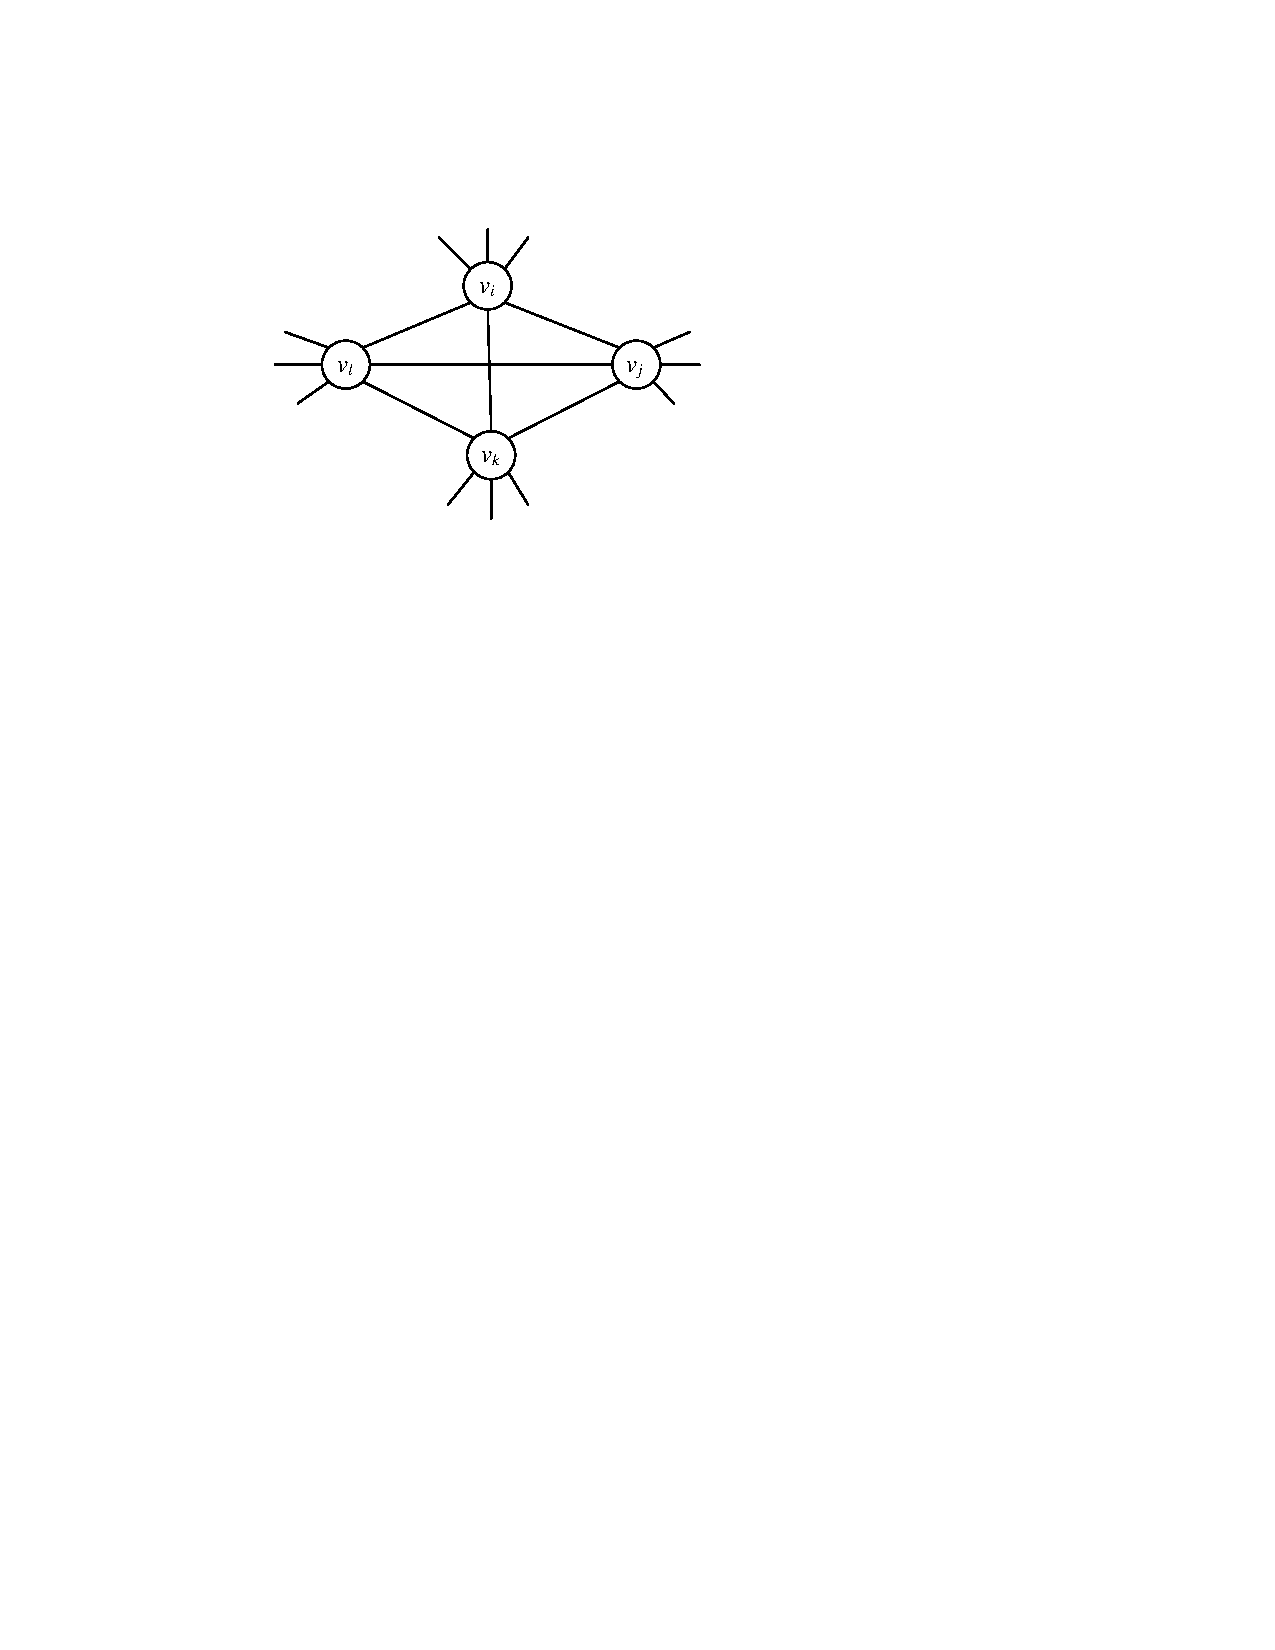
\includegraphics[width=2.2 in, height=1.5 in]{Ch3f1.pdf}
 \caption{ A fragment of a $3$-tree
 \label{fig:f3t}
}
\end{figure}


\begin{itemize}[noitemsep,nolistsep]
\item $K_{v_i,base}$ : the $k$-clique to which node $v_i$ is attached in a recursive construction of the graph $\tilde{G}$ according to the reverse sequence of the given $PES$. For the 3-tree fragment in figure \ref{fig:f3t}, assume that $K_{v_i,base}$ is the triangle (3-clique) on nodes $\{v_j, v_k, v_l\}$.
\item $K_{v_i,1}, K_{v_i,2}, \ldots, K_{v_i,k}$ : all possible $k$-cliques involving node $v_i$ when this node becomes a $k$-leaf, assuming that we started with the full $k$-tree $\tilde{G}$. Each $k$-clique is made of node $v_i$ and $k-1$ nodes in $K_{v_i,base}$. For the 3-tree in figure \ref{fig:f3t}, we may set $K_{v_i,1}=$ the triangle $(v_i,v_j,v_k)$, $K_{v_i,2}=$ the triangle $(v_i,v_j,v_l)$, $K_{v_i,3}=$ the triangle $(v_i,v_k,v_l)$.
\end{itemize}



Processing of node $v_i$ is done when all nodes in the prefix $v_1, v_2, \ldots, v_{i-1}$ have been processed and deleted, and thus node $v_i$ becomes a $k$-leaf (also called a simplicial node) in the current reduced graph. Information about certain subgraphs on the deleted nodes are maintained in special tables associated with the $k$-cliques $K_{v_i,base}, K_{v_i,1}, \ldots, K_{v_i, k}$. We use $T_{v_i,\alpha}$ to denote the table associated with clique $K_{v_i,\alpha}$ where $\alpha=base, 1, 2, \ldots, k$.

\begin{example}
\normalfont
In figure \ref{fig:f32t}, if $v_a \mbox{ and }v_b$ have been deleted to make $v_i$ a simplicial node, the information about the induced subgraph on nodes $(v_a, v_b, v_i, v_j, v_k)$ is summarized in table, say, $T_{v_i,1}$ associated with clique $K_{v_i,1}=(v_i,v_j,v_k)$. $\blacksquare$
\end{example}

\begin{figure}[!htb]
\centering
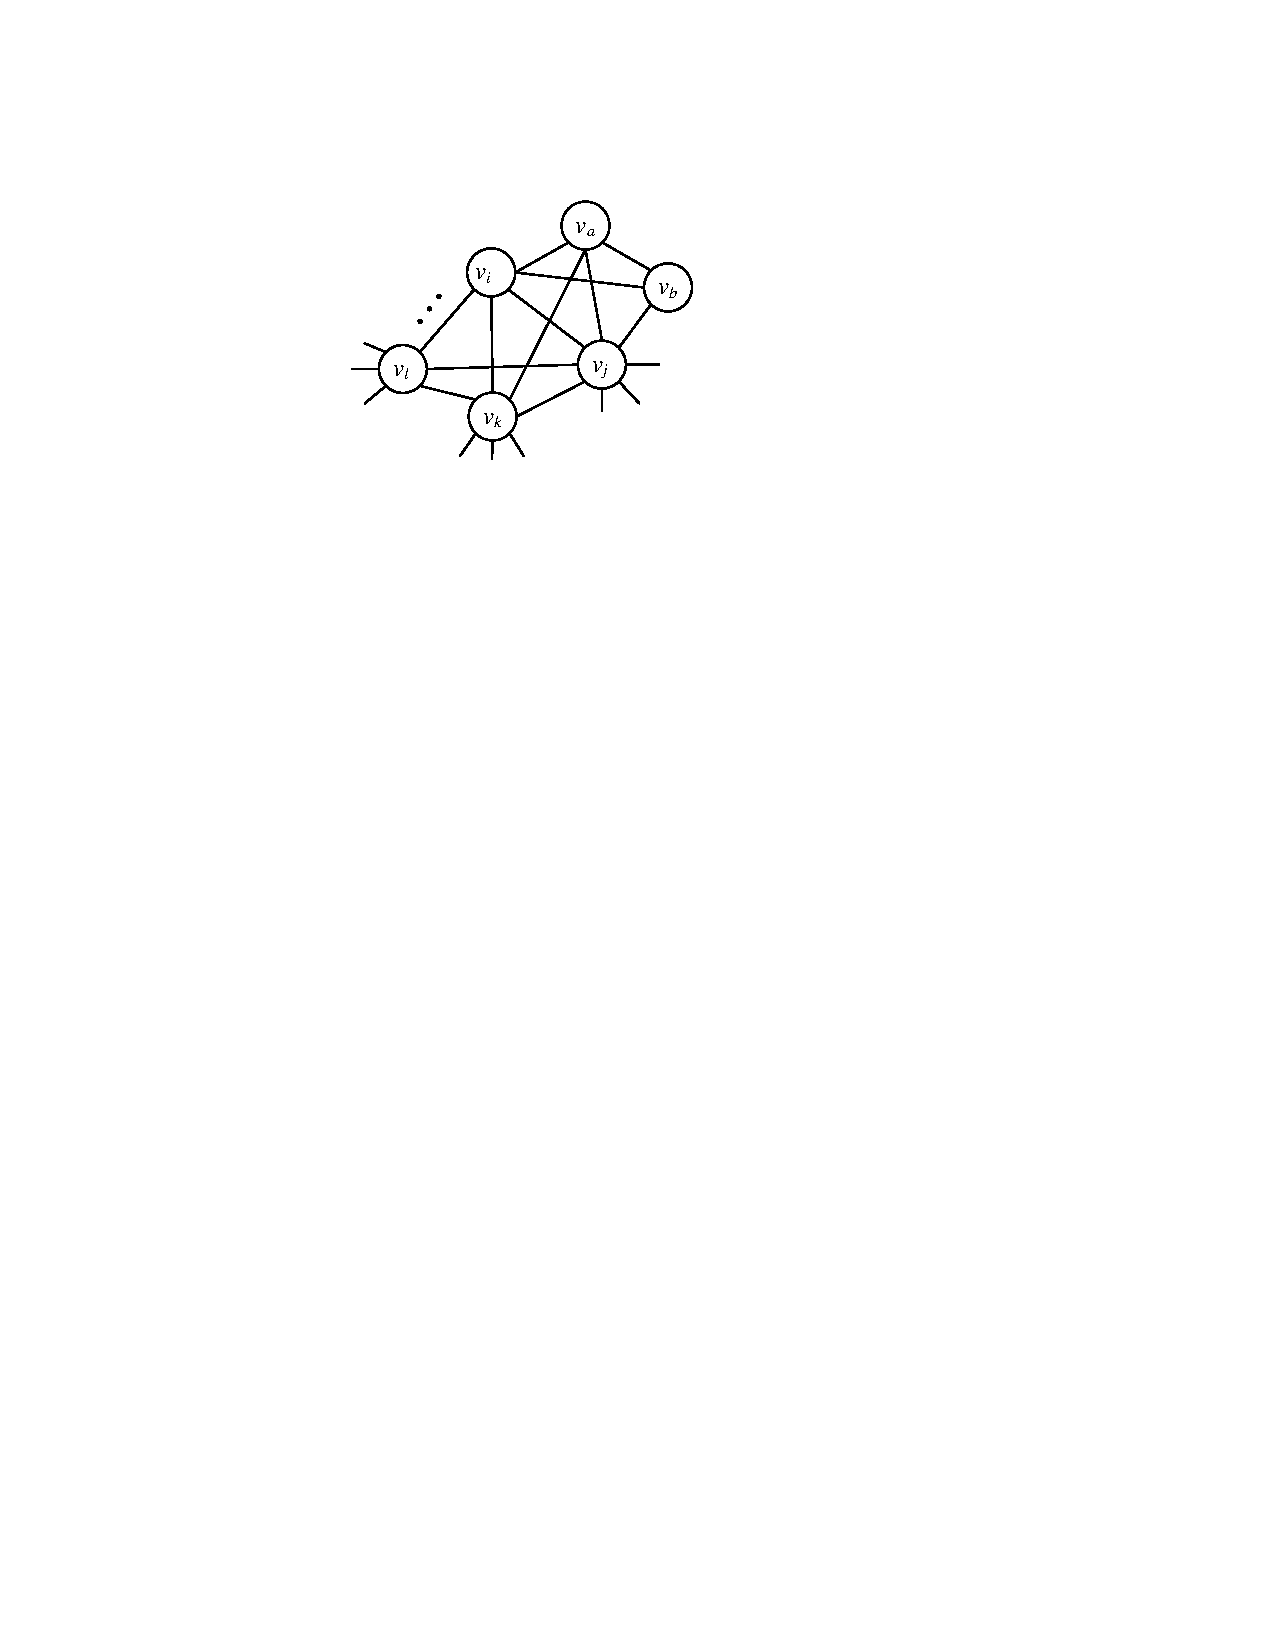
\includegraphics[width=2.4 in, height=1.5 in]{Ch3f2.pdf}
 \caption{ A 3-tree fragment
 \label{fig:f32t}
}
\end{figure}
In the above example, we say that the induced subgraph  on nodes $(v_a, v_b, v_i, v_j, v_k)$ is \textit{reduced onto} the clique $(v_i, v_j, v_k)$. Thus, prior to processing node $v_i$, the algorithm maintains in each table $T_{v_i,\alpha}$ (where $\alpha=base, 1, 2, \ldots, k$) information about a subgraph, denoted $G_{v_i,\alpha}$, that has been reduced onto the clique $K_{v_i,\alpha}$. Initially, each such table $T_{v_i,\alpha}$ stores information about the $k$-clique $K_{v_i,\alpha}$ itself. More specifically, the algorithm stores information about some useful \textbf{network states} of the graph $G_{v_i,\alpha}$ in the table $T_{v_i,\alpha}$. 

We recall from section \ref{ch1:nls}, that a network state of a graph specifies for each node $x$ in the graph a position (i.e., a \textit{grid rectangle}) in $x$'s locality set $Loc(x)$. A network state of a subgraph $G_{v_i,\alpha}$ is \textbf{good} if it appears in some operating state of the entire UWSN $G$. 

Storing and processing all possible useful network states of a graph $G_{v_i,\alpha}$ requires space and processing time that grow exponentially with the number of nodes in the graph. To gain efficiency in this regard, the algorithm consolidates information about many network states that are considered of the same \textit{type}. To explain the approach taken by the algorithm we introduce the following definition.

\begin{definition}[\textbf{state types of the $A$-$CONN$ problem}]
Let $G_{v_i,\alpha}$ be a subgraph reduced onto the clique $K_{v_i,\alpha}$. Denote by $V_{v_i,\alpha}$ the set of nodes of the graph $G_{v_i,\alpha}$. Let $S=\{v_a[i_a] :v_a\in V_{v_i,\alpha}, i_a \in Loc(v_a)\}$ be a network state of $G_{v_i,\alpha}$. Then\\
\centerline{
$A\mbox{-}type(S)=(V_1^{\loc(V_1)}, V_2^{\loc(V_2)}, \ldots, V_r^{\loc(V_r)})$}

if the following holds:
\begin{enumerate}
\item $\{V_1, V_2, \ldots, V_r \}$ is a partition of the nodes in $V_{v_i,\alpha}$. Thus, $1\leq r\leq|V_{v_i,\alpha}|$ where $r=1$ if all nodes of $V_{v_i,\alpha}$ appears in one part, and $r=|V_{v_i,\alpha}|$ if each node of $V_{v_i,\alpha}$ appears in a separate part of the partition.
\item For each part $V_j\subseteq V_{v_i,\alpha}$, $Loc(V_j)$ is a vector where the first (second, third, and so on) elements specifies a position (i.e. a grid rectangle) of the first (respectively, second, third, and so on) node in $V_j$. Thus, $V_j^{Loc(V_j)}$ specifies a subset of the network state $S$.
\item Nodes belong to one part of the partition if and only if they belong to the same connected component in the state $S$. $\blacksquare$
\end{enumerate}
\end{definition}
\begin{example}
\normalfont
In figure \ref{fig:f32t}, denote by $G_{v_i,1}$ the graph induced on the set of nodes $\{v_a, v_b, v_i, v_j,v_k\}$. $G_{v_i,1}$ is reduced onto the clique $K_{v_i,1}=$ the triangle $(v_i,v_j,v_k)$. Suppose that $S=\{v_a[1], v_b[2], v_i[1], v_j[2], v_k[3]\}$ is a possible network state of $G_{v_i,1}$ where square brackets enclose possible node positions. Moreover, suppose that $S$ has 2 connected components : $\{v_a, v_b, v_i\}$ and $\{v_j, v_k\}$. Then state $S$ is good for the $\ACONN$ problem since it does not leave any processed sensing node (nodes $v_a$ and $v_b$) disconnected from all nodes of the triangle $\{v_i, v_j, v_k\}$. State $S$ induces the partition $(\{v_i\}, \{v_j,v_k\})$ on the triangle $(v_i,v_j,v_k)$. Thus, $A\mbox{-}type(S)=(\{v_i\}^{(1)}, \{v_j,v_k\}^{(2,3)})$. $\blacksquare$
\end{example}


Each table $T_{v_i,\alpha}$, where $\alpha=base, 1, 2, \ldots, k$, provides a key-value mapping where
\begin{itemize}[noitemsep]
\item each key is a network state type of the graph $G_{v_i,\alpha}$ where $G_{v_i,\alpha}$ has been reduced thus far onto clique $K_{v_i,\alpha}$, and
\item each value is the probability of obtaining a network state of $G_{v_i,\alpha}$ having the $A\mbox{-}type$ given by the corresponding key.
\end{itemize}

\begin{example}
\normalfont
Figure \ref{fig:3t} illustrates a probabilistic network $G$ on $9$ nodes. The network has the topology of a $3$-tree. The algorithm associates edge with each triangle a table. Each triangle can be partitioned in 5 different ways (since, the Bell number $B_3=5$). For example, the $5$ partitions of triangle $(v_1,v_2,v_3)$  are $\{v_1,v_2,v_3\}, \{v_1,v_2\}\{v_3\}, \{v_1,v_3\}\{v_2\},\{v_2,v_3\}\{v_1\}$ and $\{v_1\}\{v_2\}\{v_3\} $. The number of possible keys that appear in the table of triangle $(v_1,v_2,v_3)$ is $5 \times 6 \times 6 \times 3$ since $B_3=5, |Loc(v_1)|=6$, $|Loc(v_2)|=6$ and $|Loc(v_3)|=3$. $\blacksquare$
\end{example}
\begin{figure}[htbp]
\centering
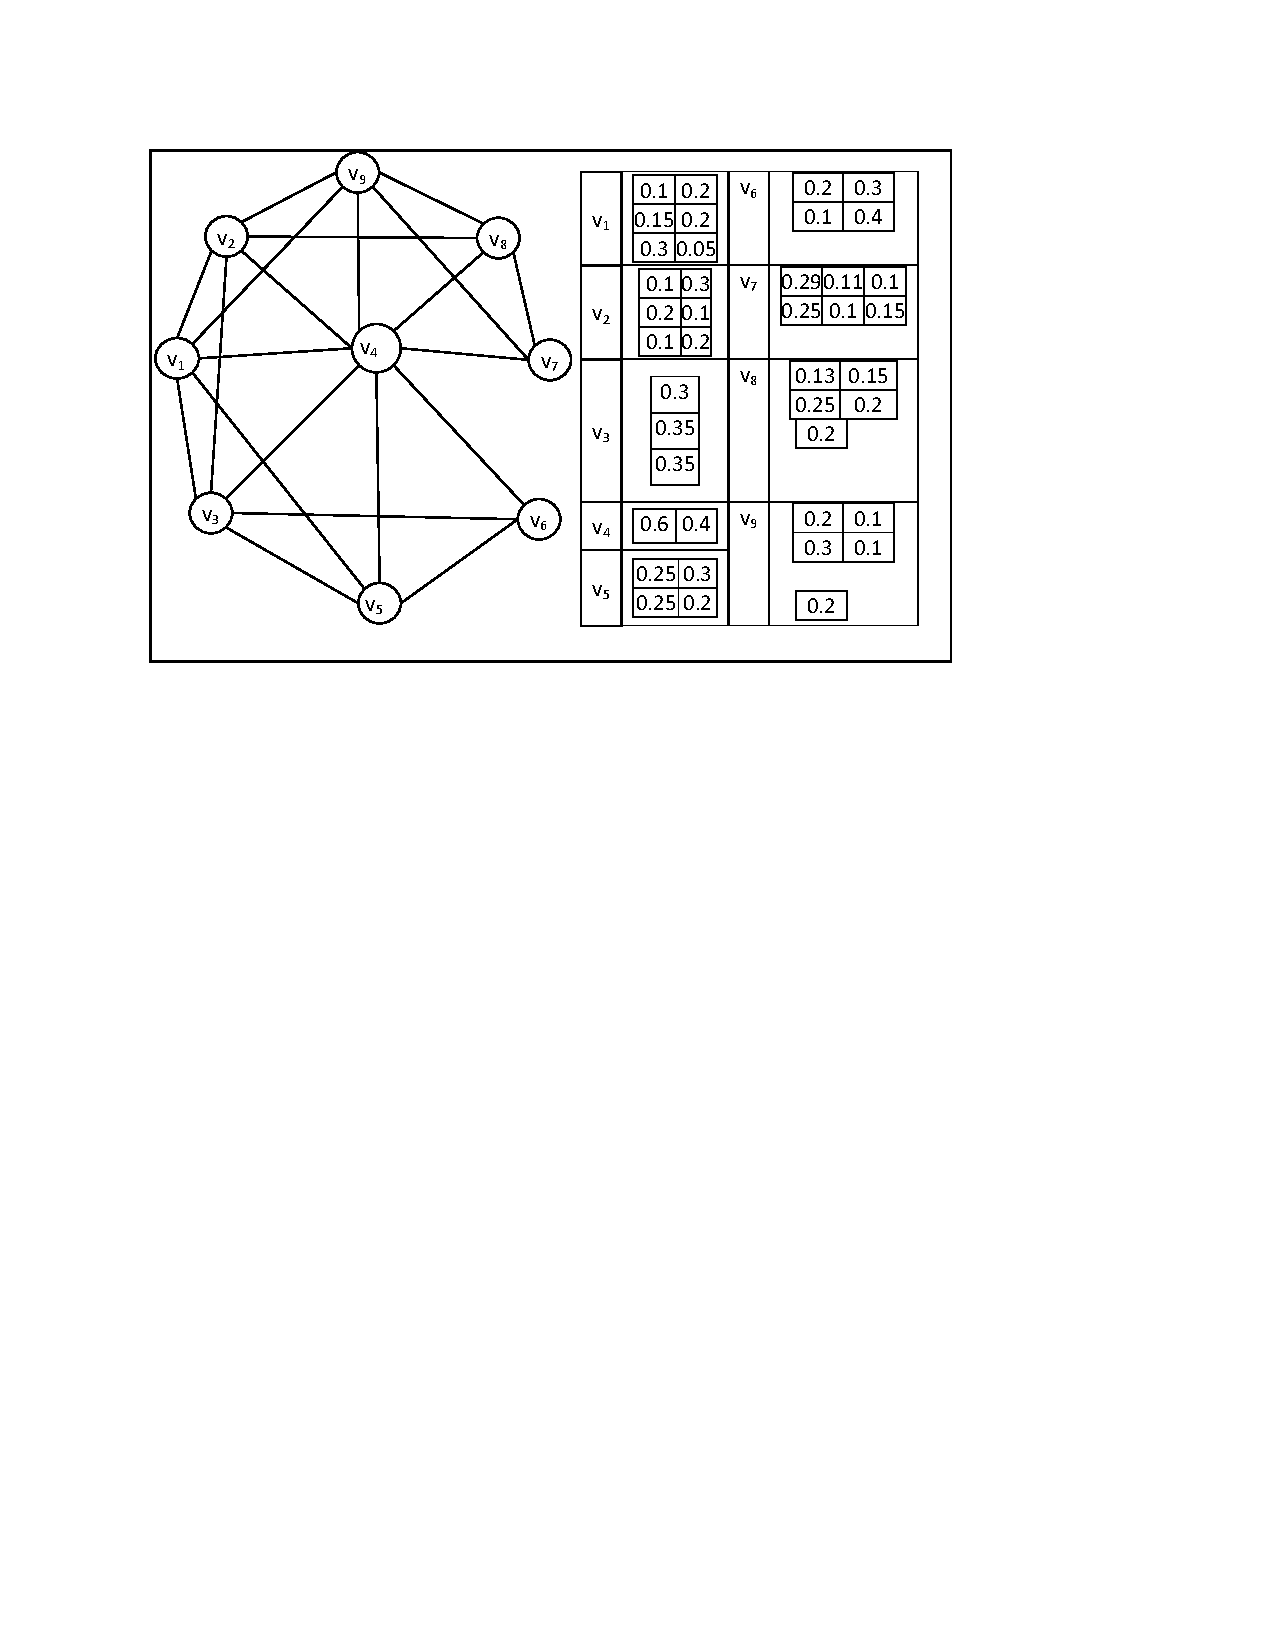
\includegraphics[width=4 in, height=2.4 in]{relay1.pdf}
 \caption{ A UWSN modelled by a $3$-tree}
 \label{fig:3t}
\end{figure}

\section{Algorithm Organization}
\label{sec:algorg}

The overall algorithm is organized around $3$ functions : a top level main function (Algorithm \ref{Alg:fmain1}), a middle level table merge function (Algorithm \ref{ch3:fmerge}: $t\_merge$), and a low level partition merge function (Algorithm \ref{ch3:fmpar}: $p\_merge$).\\\\
%
The highlights of each function are explained below:
\begin{itemize}
\item Function Main (Algorithm \ref{Alg:fmain1}): This function reduces the structure of the probabilistic network (and the underlying partial $k$-tree) $G$ by iteratively  processing and then deleting nodes according to the given $PES$, say $(v_1, v_2, \ldots, v_n)$ where $V_n=s$ (the sink node), until the network is reduced to the $k$-clique $(v_{n-k+1}, \ldots, v_n)$. Processing a node $v_i$ entails merging the tables $\{K_{v_i,\alpha} :\alpha=base, 1, 2, \ldots, k\}$.
 %
This merging phase is done by merging a sequence of pairs of tables. The middle level table merge function is used for this purpose.
%
After all iterations are done, the solution is computed from the table associated with the clique on nodes $(v_{n-k+1}, \ldots, v_n)$.
\item Function Table Merge (Algorithm \ref{ch3:fmerge}: $t\_merge$): This function takes as input a pair of tables, denoted $T_1$ and $T_2$, associated with two overlapping cliques. Roughly speaking, it performs a cross-product of $T_1$ and $T_2$; that is, it constructs a new table, denoted $T_{out}$, by processing every pair of keys: $key_1\in T_1$ and $key_2\in T_2$. To process the partition parts of the keys $P_1 \in key_1$ and $P_2 \in key_2$, the function calls the low level partition merge function.
\item Function Partition Merge (Algorithm \ref{ch3:fmpar}: $p\_merge$): This function takes two partitions $P_1 \in key_1 \in T_1$ and $P_2 \in key_2 \in T_2$, as explained above, and computes a partition $P_{out}$ that is a valid partition of a key in the merged table $T$.
\end{itemize} 
\subsection{Function Main}
\label{subsub:Main}

Algorithm \ref{Alg:fmain1} presents the main steps of the top level main function. The algorithm takes as input a probabilistic network $G=(V, E_G, Loc, p)$ that has the topology of a partial $k$-tree, also denoted $G$, and a $PES$ of $G$. It computes the exact $\ACONN$ of $G$ in $Conn(G)$. For simplicity of presenting the pseudo-code, we assume that the nodes $V=V_{sense}$ in $G$ are labelled so that the $PES=(v_1, v_2, \ldots, v_n)$ and $v_n=s$ (the sink node).

The function has 3 main parts, as explained below.

\textbf{Initialization (Step 1):} We initialize a table $T_H$ associated with each $k$-clique $H$ in the full $k$-tree $\tilde{G}$. In particular, for each possible state type, say $k$, of a network state on the nodes of $H$, we set a key-value entry in $T_H$ where the key is $k$, and the value is the probability of obtaining a network state of $H$ of that type. If $G$ is a strict partial $k$-tree (So, $G \neq$ $\tilde{G}$ ) then some edges of $H$ may be missing. However, the above initialization approach is still applicable.

We remark that initializing table $T_H$ for a $k$-clique $H$ can be done as follows.
\begin{enumerate}
\item First, we construct for each edge $e=\{x,y\}$ in $H$ an exhaustive table $T_e$. As explained above, $T_e$ contains key-value mappings. Each key has the form $A\mbox{-}type(S)$ for a possible state $S$ on $\{x,y\}$ (e.g., $(\{x\}^{(1)} \{y\}^{(1)}), \{x,y\}^{(1,1)}, \ldots$). The value associated with $A\mbox{-}type(S)$ is the probability of obtaining a network state of this $A\mbox{-}type$ over the edge $e$.
\item Second, we compute (using function $t\_merge \mbox{ and }p\_merge$) the cross product of all tables associated with all edges in the $k$-clique $H$.
\end{enumerate}
%The initialization phase is done iteratively as follows.We first generate all state types for 1-cliques (i.e., isolated nodes), and then use them to generate all states types for 2-cliques, and then use them to generate all state types for 3-cliques, and so on. That is, we make use of the observation that all state types for $k$-cliques, $k\ge 2$, can be generated from all state types of smaller cliques.

\begin{algorithm} [!htb]
\Indm
\KwIn{ An instance of the $A$-$CONN$ problem where $G$ has a partial $k$-tree topology with a given $PES$=$(v_1, v_2, \ldots, v_n)$}
\KwOut{ $Conn(G)$}
\textbf {Notation:} $Temp$ is a temporary table.\\
\nwline
\Indp
\nl \textbf{Initialization:} initialize a table $T_H$ for each $k$-clique $H$ of $G$.  
\iin{1.15} $T_H$ contains all possible state types on nodes of $H$.\\
\nl\For{$(i=1,2, \ldots,|V|-k)$}
{
\nl $ Temp=T_{v_i,1}$  \\
 \nl \For{$(j=2, 3, \ldots, k)$}
 {
  \nl $Temp=t\_merge(Temp,T_{v_i,j})$\\
 }
 \nl$T_{v_i,base}=t\_merge(Temp,T_{v_i,base})$\\
 \nl \ForEach{$(key \in T_{v_i,base})$}
 {
 \nl \If{$(v_i$ is a singleton part of $key)$}
 {
 \nl delete $key$ from $T_{v_i,base}$
 }
  \Else{
  \nl delete $v_i$ and its associated position from $key$
  }
 }
}

\nl \Return{$Conn(G)$} $=\sum \begin{array}[t]{l}
 \mbox{values in table }T_{v_{n-k},base} \mbox{ corresponding to state types}\\ \mbox{that have exactly one connected component}
\end{array}$

\caption{Function Main$(G$, $PES)$}
\label{Alg:fmain1}
\end{algorithm}
\textbf{Main Loop (Step 2):} The main loop has two parts. The first part (Steps 2 to 6) iteratively processes and deletes nodes in the $PES$. Processing a node $v_i$ entails merging a sequence of tables $(T_{v_i,\alpha}: \alpha=base, 1, 2, \ldots,k)$ into one table. This step is carried by merging a pair of tables at a time. We use table $Temp$ to store intermediate results. We store the final result in table $T_{v_i,base}$. 

The second part (Steps 7 to 10) removes \textbf{bad} state types from table $T_{v_i,base}$. For the $\ACONN$ problem, a state $S$ of the graph $G_{v_i,base}$ reduced onto the $k$-clique $K_{v_i,base}$ is considered bad at this stage if node $v_i$ appears as a singleton part in the partition specified by $A\mbox{-}type(S)$.
 
This badness holds because $K_{v_i,base}$ is a separator clique in $G$. So, if $v_i$ appears disconnected from the nodes in $K_{v_i,base}$ in any network state $S$ then $S$ can not be extended to an operating state of the entire network. On the other hand, if $A\mbox{-}type(S)$ is not bad, then step 10 just removes node $v_i$ and its associated position from $A\mbox{-}type(S)$.

\begin{example}
\normalfont

Figure \ref{fig:3t} illustrates a 3-tree that has a $PES=(v_6, v_5, v_7, v_8, v_9, v_4)$. the main loop processes node $v_6$ by merging tables $T_{v_6,1}$ on nodes $\{v_4, v_5, v_6\}$, $T_{v_6,2}$ on nodes $\{v_3, v_5, v_6\}$, $T_{v_6,3}$ on nodes $\{v_3, v_4, v_6\}$, and $T_{v_6,base}$ on nodes $\{v_3, v_4, v_5\}$ into one table stored in $T_{v_i,base}$. $\blacksquare$
\end{example}

\textbf{Termination (Step 11):} The main loop finishes after processing node $v_{n-k}$. The resulting table $T_{v_{n-k},base}$  corresponds to the $k$-clique $H$ on nodes $(v_{n-k+1}, \ldots, v_n)$. Any state type where all nodes of $H$ appear in one connected component corresponds to a set of operating network states of the entire network . Thus, we return the sum of probabilities of all such state types.


\subsection{Function Table Merge}
\label{subsub:Mrg}
\begin{algorithm}[htbd]
\Indm  
\KwIn{ Two tables $T_1$ and $T_2$ that may share common nodes}
\KwOut{A merged table $T_{out}$}
\nwline
\Indp
\nl \textbf{Initialization:} Clear table $T_{out}$\\
\nl \textbf{set} $C=$ the set of common nodes between $T_1$ and $T_2$\\
 \nl \ForEach{$($pair of state types $key_1 \in T_1$ and $key_2 \in T_2 )$}
 {
 \nl \If{$($any node in $C$ lies in two different positions in $key_1 \mbox{ and } key_2)$} {
 \nl\textbf{ continue}}
 \nl \textbf{set} $key_{out}=$ the state type obtained from node positions in $key_1$ and $key_2$,
 \iin{0.9}  and the partition computed by $p\_merge(key_1,key_2)$\\
 \nl \textbf{set} $p_{out}=T_1(key_1)\times T_2(key_2)$ adjusted to take the effect of common nodes in 
  \iin{0.7} $C$ into consideration\\
 \nl \If{$(key_{out} \in T_{out})$} {
\nl update $T_{out}(k_{out})\plusEqual p_{out}$ 
 }
 \Else{
\nl \textbf{set} $T_{out}(key_{out})=p_{out}$ 
 } 
  }
  
\nl \Return {$T_{out}$}
 \caption{Function $t\_merge$($T_1,T_2$)}
 \label{ch3:fmerge}
\end{algorithm}

Algorithm \ref{ch3:fmerge} illustrates the main steps of the middle level table merge function. We recall that $t\_merge$ is called from the main function to merge two tables, denoted $T_1$ and $T_2$, that may have a set $C$ of common nodes (i.e., $V(T_1) \cap V(T_2) \neq \emptyset$).
Each table $T_i, i=1, 2,$ stores information about some subgraph, $G_i$, that has been reduced onto some $k$-clique, $K_i$. 
Table merging is done by processing each pair of state types (i.e., table keys) $key_1 \in T_1 \mbox{ and } key_2 \in T_2$. Processing state types $key_1$ and $key_2$ results in a new state type, denoted $key_{out}$, and an associated probability, denoted $p_{out}$. \\


To explain the processing on $key_1$ and $key_2$, consider two network states: $S_i, i=1, 2,$ where $S_i$ is a network state of the subgraph $G_i$ (reduced onto clique $K_i$) and $key_i=A\mbox{-}type(S_i)$.
Merging $S_1$ and $S_2$ gives the union $S_1\cup S_2$. This union is possible only if each common node in $C$ assumes the same position in both of $S_1$ and $S_2$. If the union is possible then the desired state type $key_{out}=A\mbox{-}type(S_1\cup S_2)$, and the desired $p_{out}$ is the probability that a state of $key_{out}$ arises in the graph $G_1 \cup G_2$. 

As explained in the next section, the $A\mbox{-}type(S_1\cup S_2)$ can be deduced from node position information in $key_1=A\mbox{-}type(S_1)$ and $key_2=A\mbox{-}type(S_2)$. The probability $p_{out}$ is the product $T_1(key_1)\times T_2(key_2)$ divided by a correction term $=\prod (p_x(i):x[i] \mbox{ is common between } key_1 \mbox{ and } key_2)$.


\subsection{Function Partition Merge }
\label{subsub:fMpar}
As in the previous section, for $\alpha=1, 2,$ let $T_{v_i,\alpha}$ be a table containing summary information about useful network states 
of the graph $G_{v_i,\alpha}$ that has been reduced onto the clique $K_{v_i,\alpha}$. We use the simplified notation $T_1=T_{v_i,1}, \mbox{ and } T_2=T_{v_i,2}$. A core operation performed by the function presented in the previous section is to process every pair of \textit{keys} ($key_1,key_2$) where $key_1\in T_1$ and $key_2\in T_2$. This operation results in a new key, denoted $key_{out}$. To compute $key_{out}$, we need to compute the partition on the set of nodes of $K_{v_i,1}$ union $K_{v_i,2}$ (i.e. $V(K_{v_i,1})\cup V(K_{v_i,2})$) that results by merging partition $P_1$ of $key_1$ with partition $P_2$ of $key_2$.

In this section, we discuss an algorithm to merge partition $P_1$ and $P_2$ to obtain $P_{out}$. We illustrate this merging step using the example in figure \ref{fig:ftc}.

\begin{example}
\normalfont
In figure \ref{fig:ftc}, $P_1=\{\{v_1\}\{v_2,v_3\}\{v_4,v_5\}\}$ and $P_2=\{\{v_4,v_5,v_6\}\{v_7,v_8\}\}$. Thus,  $P_{out}=\{\{v_1\}\{v_2,v_3\}\{v_4,v_5,v_6\}\{v_7,v_8\}\}$. $\blacksquare$
\end{example}


\begin{figure}[!htb]
\centering
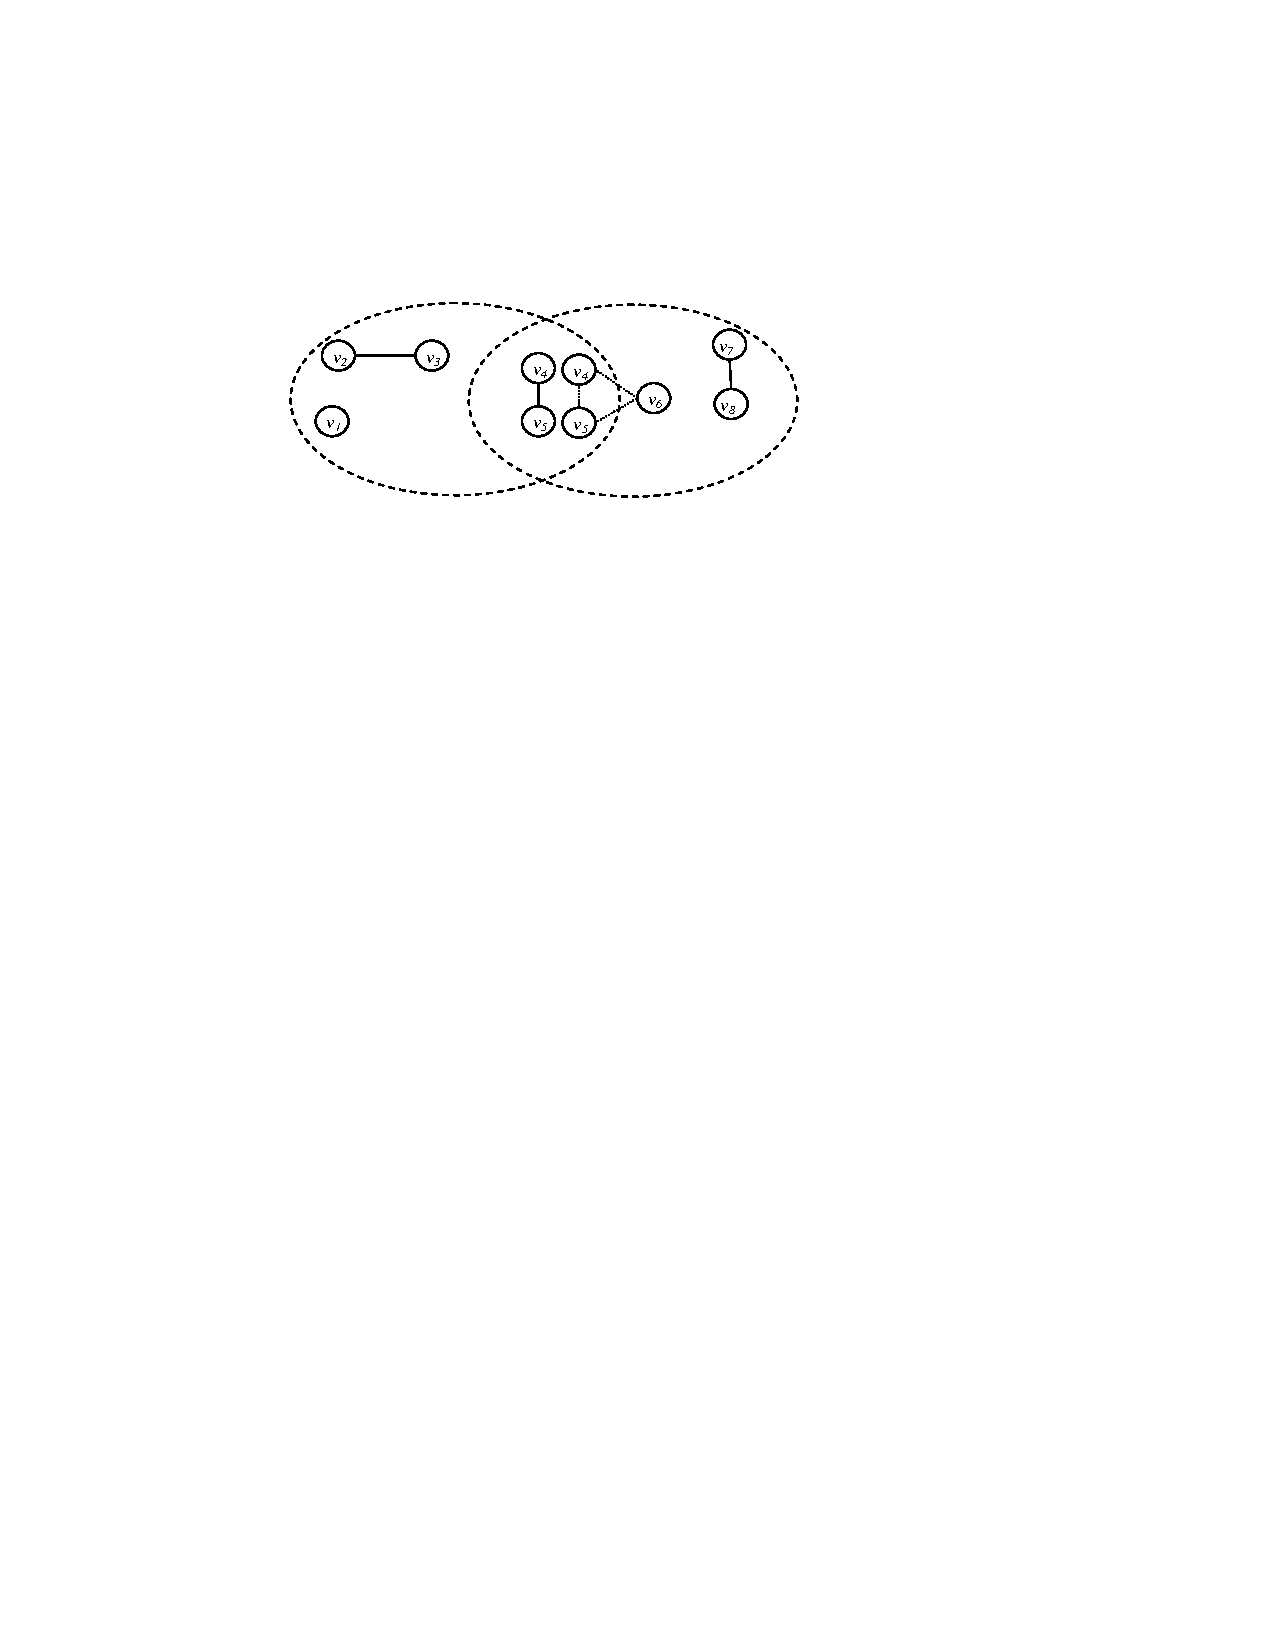
\includegraphics[width=3 in, height=1.3 in]{Ch3fpmarge.pdf}
 \caption{ Merging two partitions}.
 \label{fig:ftc}
\end{figure}

Our method of computing $P_{out}$ can be summarized as follows. Each partition (e.g. $P_1$ or $P_2$) is represented by a list of sets (a list is an ordered container). Each part within a partition is represented as a set of nodes. 


First, we put all parts of $P_1$ and $P_2$ in one partition. In function $p\_merge$ (Algorithm \ref{ch3:fmpar}) we choose to put all parts in $P_1$ (steps 1 and 2). Second, we process each pair of parts in $P_1$ by merging them into one part if there is at least one common node. If two parts are merged together, then both parts are deleted from the ordered list $P_1$ and their union is placed at the beginning of $P_1$. Processing of pairs of parts in the updated $P_1$ then restarts from the beginning of $P_1$. Processing finishes when all pairs in the ordered list $P_1$ are considered.


% The merging partitions is mainly done using the union operation by mapr function. The mpar function takes as input two partitions $P_1$, $P_2$ and merge them into one partition $P$.
%
%In more details,  
%\begin{itemize}[noitemsep,nolistsep]
%\item Steps $1$-$2:$ adds all the sets of $P_2$ to $P_1$.
%\item Steps $3$-$4:$ selects two sets $s^*$ and $t^*$ from partition $P_1$ 
%\item Step $5$: checks whether or not they are disjoint . If they are  not disjoint then it will go to step 6 otherwise it will return to step 4.
%\item Step $6:$ delete $s^*$ from $P_1$.
%\item Step $7:$ computes the union of $s^*$ and $t^*$ and insert it at the beginning of partition $P_1$.
%\item Step $8:$ delete $t^*$ from $P_1$.
%\item Steps $9$-$10:$ set the iterator to the beginning of $P_1$ and return to step 5.
%\item Step $11:$ assign $P_1$ to $P$ and finally the algorithm return $P$.
%\end{itemize}


\begin{algorithm}[htpd]
\KwIn{Two partitions $P_1$ and $P_2$}
\KwOut{A partition $P$}
\textbf{Notation:} $s$ and $t$ are two set iterators and their corresponding set are indicated by $s^*$ and $t^*$.\\ 
\nl \ForEach{$($ set $s^*$ in $P_2)$}
{
\nl $P_1.push\_back(s^*)$
}
\nl \For{ $(s=P_1.begin()$; $s \neq P_1.end()$;  $++s)$}
{
\nl \For{ $(t=s.next()$; $t \neq P_1.end()$; $++t)$}
{
 \nl \If{$(s^*\cap t^* \neq \emptyset)$}
  {
\nl  	$  P_1.push\_front(s^*\cup t^*$) \\
\nl$P_1.delete(s^*)$\\
  \nl $P_1.delete(t^*)$\\
  \nl $s=P_1.begin()$\\
   \nl$break$\\
  }
}
}
\nl set $P=P_1$\\
\Return{P}
\caption{function $p\_merge(P_1$, $P_2)$}
\label{ch3:fmpar}
\end{algorithm}

\section{Example Tables}
\begin{example}
\normalfont
In figure \ref{fig:table1}, two keys (state types)
$key_1=(\{v_1,v_2\}^{(1,1)}\{v_3\}^{(2)})$  and $key_2=(\{v_1\}^{(1)}\{v_3,v_4\}^{(2,1)})$ belong to tables $T_1$ and $T_2$ respectively. The two keys can be merged together since the common nodes $v_1$ and $v_3$ assume the same positions $v_1[1] \mbox{ and } v_3[2]$ in both keys. Function partition merge returns the merged partition $(\{v_1,v_2\}\{v_3,v_4\})$. Thus, function $t\mbox{-}merge$ computes $k_{out}=(\{v_1,v_2\}^{(1,1)}\{v_3,v_4\}^{(2,1)})$. Now, assume that $p_{v_1}(1)=0.1 \mbox{ and }p_{v_3}(2)=0.2$. Then function $t\_merge$ computes $p_{out}= \frac{0.002\times 0.008}{0.1\times 0.2}=0.0008$, as shown.$\blacksquare$
\end{example}

\begin{figure}[!htb]
\centering
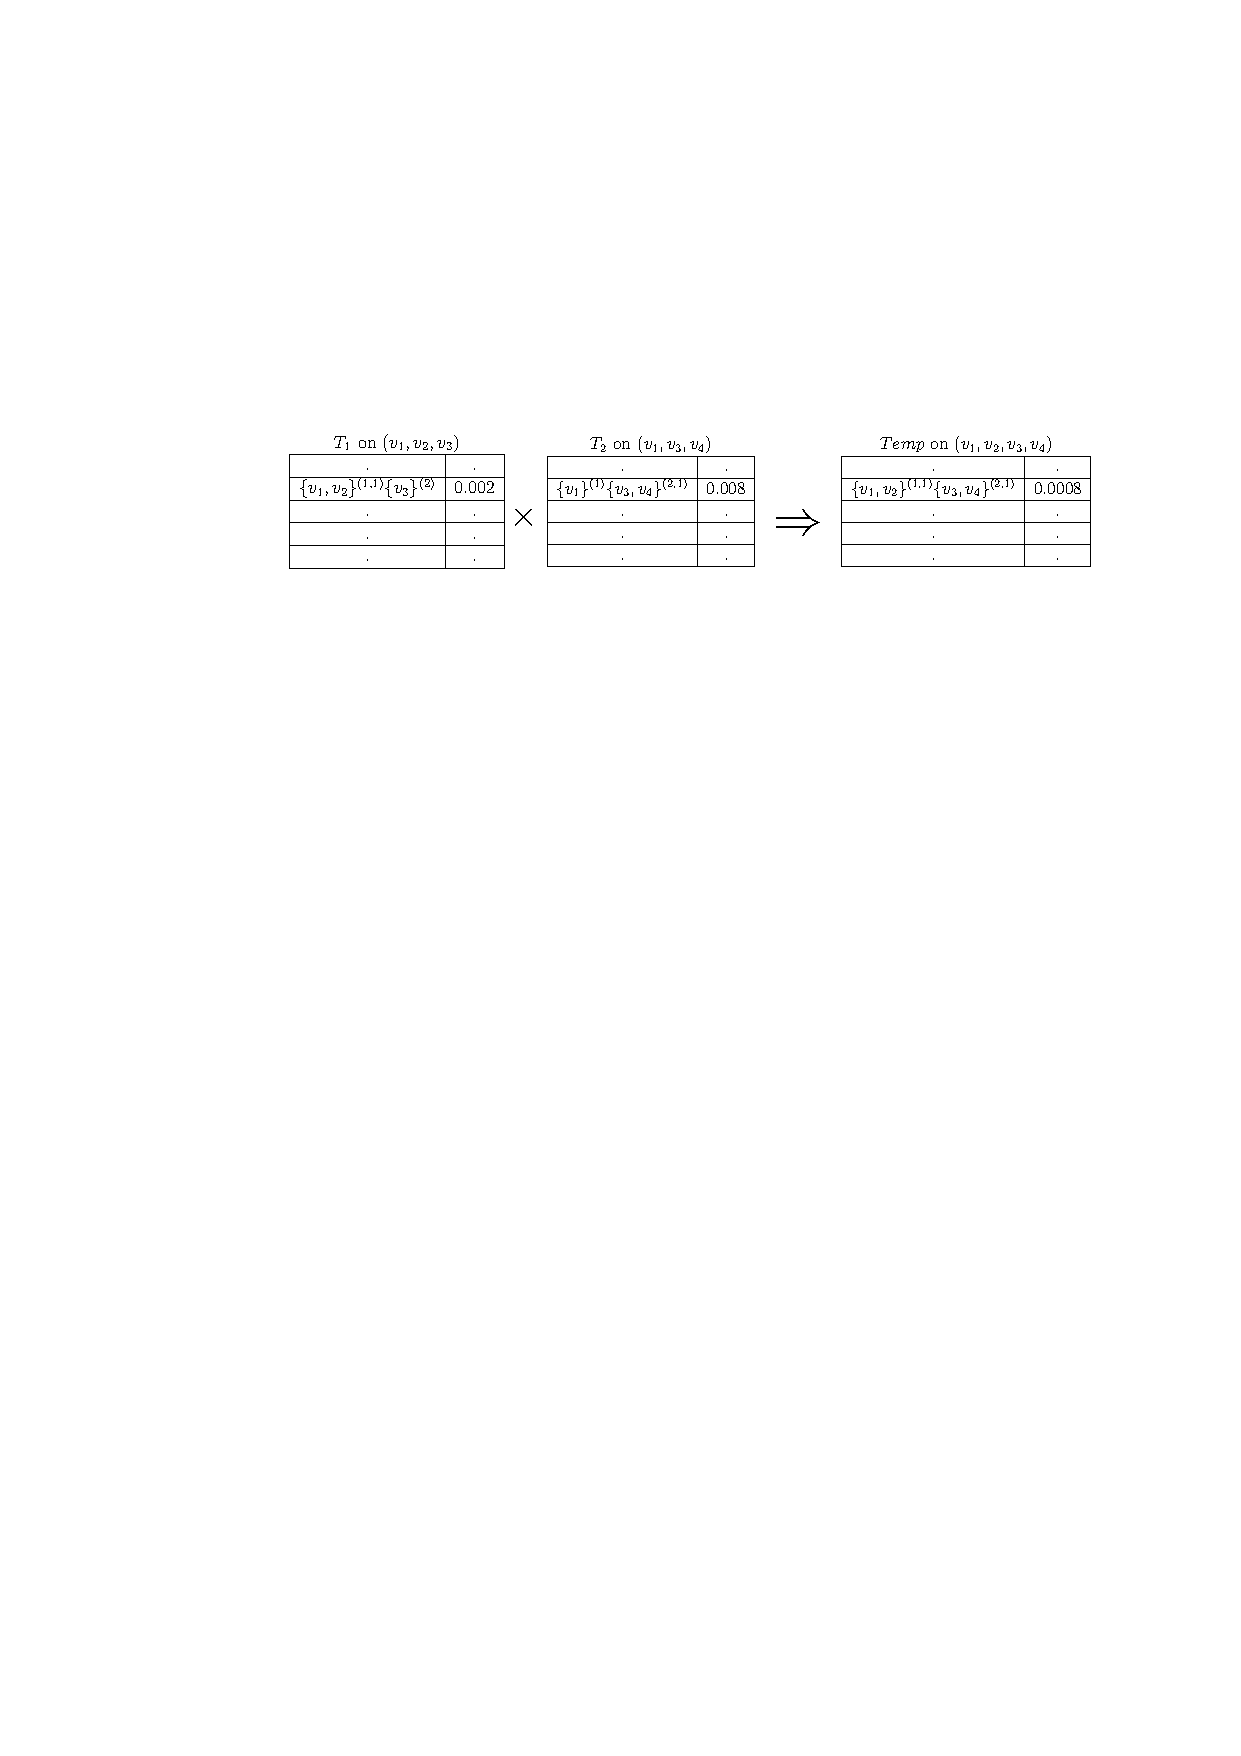
\includegraphics[width=5 in, height=1.2 in]{Table11.pdf}
 \caption{ Merging two tables}.
 \label{fig:table1}
\end{figure}

\begin{example}
\normalfont
Figure \ref{fig:table2} illustrates the operation of the second part of the main loop of function Main in the iteration where node $v_1$ is processed. The table on the left represents $T_{v_i,base}$ after the first part of the main loop finishes. Key $\{v_1,v_2\}^{(1,1)}\{v_3,v_4\}^{(2,1)}$ is good in $T_{v_i,base}$ since $v_1$ is connected to $v_2$ in any network state of this type. Hence, node $v_1$ and its associated position can be deleted from the key. The reduced key appears in the updated $T_{v_i,base}$ on the right.
\end{example}

\begin{figure}[!htb]
\centering
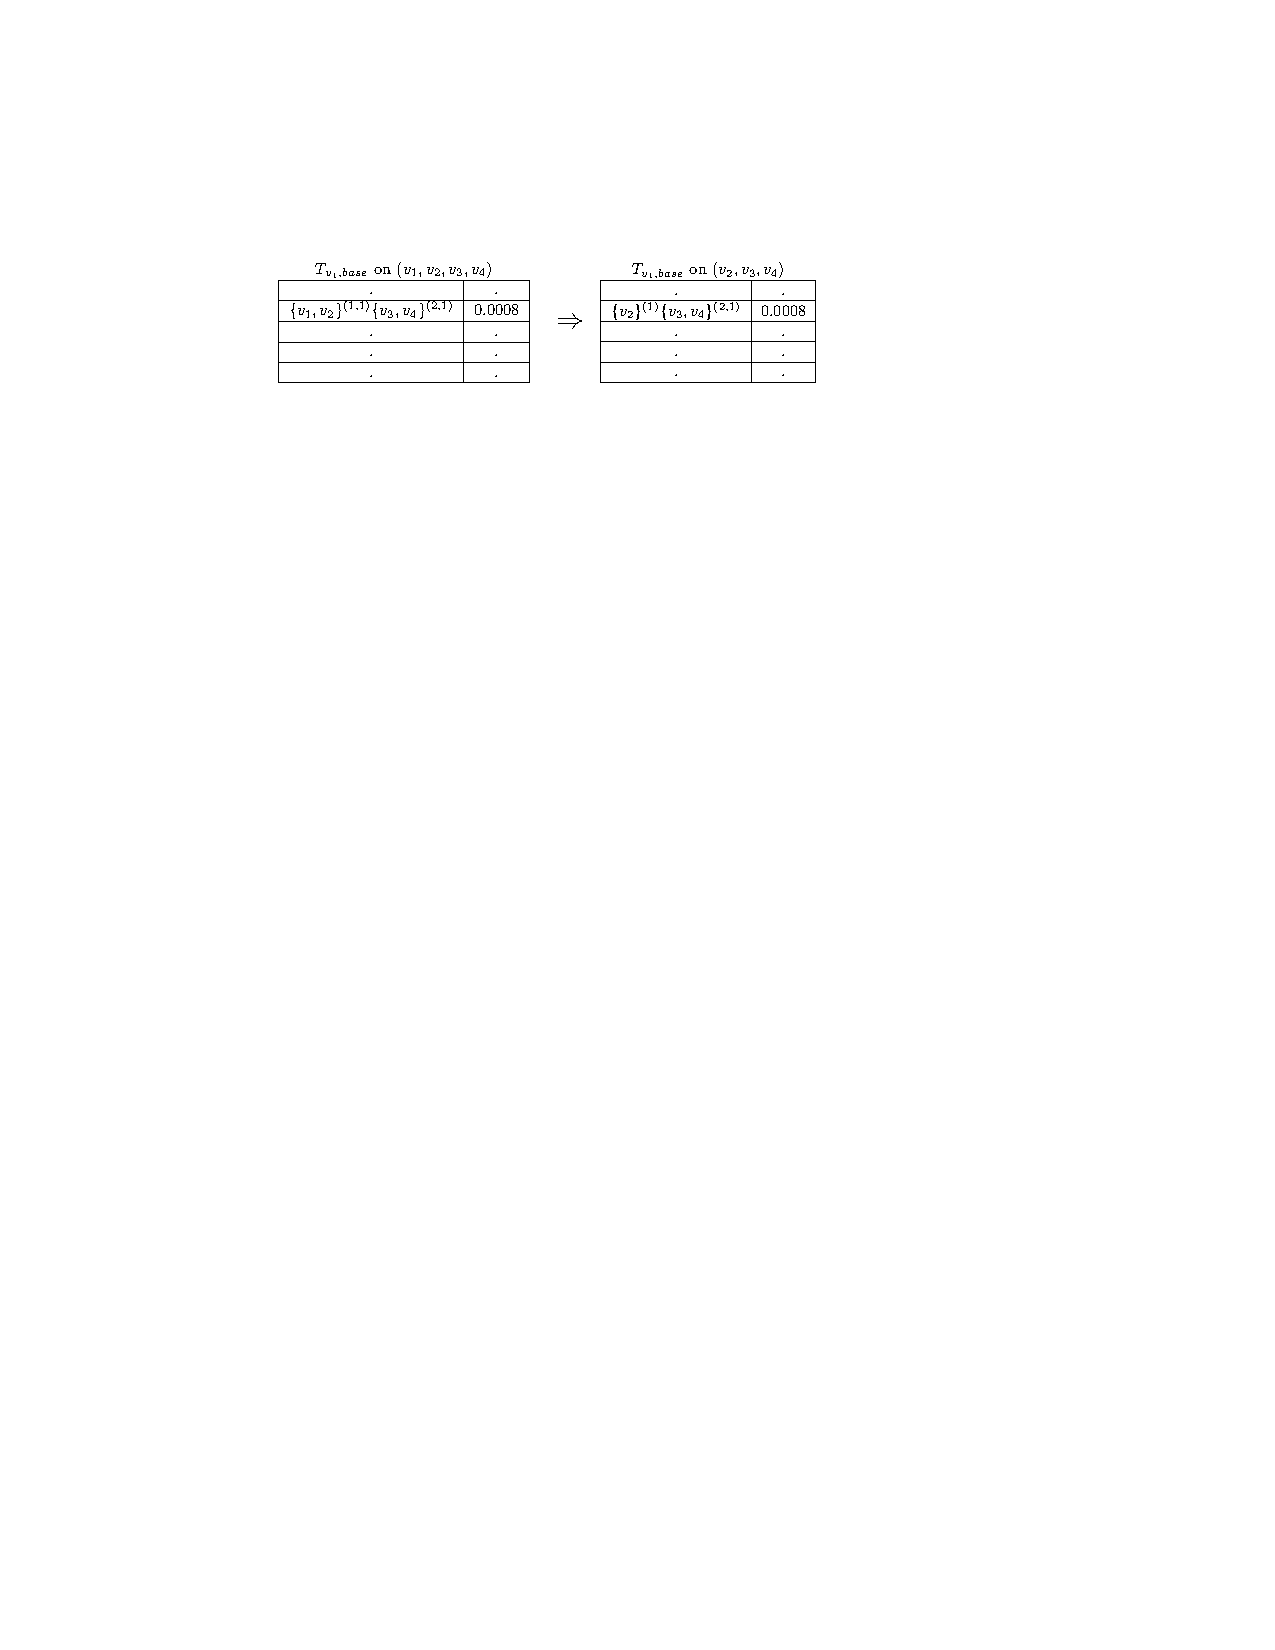
\includegraphics[width=3.5 in, height=1.1 in]{Table111.pdf}
 \caption{ Deleting node $v_i$}.
 \label{fig:table2}
\end{figure}
\section{Correctness}
\label{Sec:crtns}
To prove correctness, we introduce the following notation and definitions.
\begin{enumerate}
\item[{\bf [D1]}]We say that a table $T_{v_i,\alpha}$ is complete with respect to a graph $G_{v_i,\alpha}$ that has been reduced onto the clique $K_{v_i,\alpha}$ if the following conditions hold:
%
\begin{itemize}
%
\item[a)] For each $key\in T_{v_i,\alpha}$, the corresponding value $T_{v_i,\alpha}(key)$ is the probability of obtaining states over the subgraph $G_{v_i,\alpha}$ of type $key$.
%
\item[b)] Each key not in $T_{v_i,\alpha}$ does not contribute to computing the solution $Conn(G)$.
\end{itemize}
%
\end{enumerate}
\nwline
We now show the following theorem.


\begin{theorem} \label{thm:correctnessch4}
\normalfont
At the start of each iteration of the main loop (Step 2) of function Main, if $v_i$ is a node in the current graph then each table $T_{v_i,\alpha}: \alpha=1, 2, \ldots, k, base$, is complete with respect to the graph $G_{v_i,\alpha}$ reduced thus far onto the clique $K_{v_i,\alpha}$.
\end{theorem}
\nwline
\textbf{Proof.}\\
\textbf{Loop Initialization:} At the start of the first iteration, $G$ contains all nodes $V$.
%
In addition, for each clique $K_{v_i,\alpha}$, the subgraph $G_{v_i,\alpha}$ reduced thus far onto the clique $K_{v_i,\alpha}$ is the clique itself (as done in Step 1 of function Main).\\
\nwline
\textbf{Loop Maintenance:} Assume the theorem holds for all possible iterations $r$, where $r\leq n-k-1$. We show that it holds in iteration $r+1$. Let $v_r$ be the $k$-leaf deleted in iteration $r$.
%
Table $T_{v_r,base}$ is the only table that may have changed between iterations $r \mbox{ and } r+1$. 
%
Thus, it suffices to show that $T_{v_r,base}$ is complete with respect to $G_{v_r,base}$. To this end, we note the following in iteration r:

\begin{itemize}
\item Steps 3 to 6 of function Main merge all tables in the set $\{ T_{v_i,\alpha}:\alpha=1, 2, \ldots, k, base \}$ into $T_{v_i,base}$.
\item The loop in Step 7 of function Main discards all bad state types over the graph $\displaystyle \bigcup_{\alpha\in  \{1, 2, \ldots, k, base\}} G_{v_i,\alpha}$. $\blacksquare$
\end{itemize}

%
Following an argument similar to the loop maintenance argument, one can show that at Step 11 in function Main, table $T_{v_{n-k},base}$ associated with the clique $T_{v_{n-k},base}$ containing the sink node is complete with respect to all nodes $V$.
%
Thus, the function returns the required solution.
\section{Running time}
\label{sec:runtym}
Let $n$ be the number of nodes in $G$, $l_{max}$ be the maximum number of locations in the locality set of any node, and $B_k$ be the $k^{th}$ Bell number.
\nwline 
\begin{theorem}\label{thm:runtym}
\normalfont
In the $\ACONN$ algorithm we have
\begin{enumerate}[noitemsep]
\item The maximum length of any table is $\in O(B_k l_{max}^k)$.
\item The worst case running time is $O(n(B_k l_{max}^k)^2)$.
\end{enumerate}
\end{theorem}
\textbf{Proof.}
\nwline
To see (1), we note that the length of each table is determined by the number of partitions of any set of $k$ nodes $(=B_k)$ times the number of different positions that the $k$ nodes can take $(\in O(l_{max}^k))$. Thus, the maximum length of any table is $O(B_k l_{max}^k)$.
\nwline
To see (2), we note that function $t\_merge$ processes $O((B_k l_{max}^k)^2)$ pairs of keys in each call. Function partition merge takes $O(k^3)$ to merge two partitions; this is a constant time for any fixed $k$. Thus, merging two tables requires $O((B_k l_{max}^k)^2)$. 

Function Main processes each node by merging a set of $k\mbox{+}1$ tables. This is done by calling function $t\_merge$ $k$ times. Thus, function Main processes each node in $O(k(B_k l_{max}^k)^2)$. Since $k$ is a constant, processing each node requires $O((B_k l_{max}^k)^2)$. The answer is obtained after processing $n\mbox{-}k$ nodes. Thus, the overall running time is $O(n(B_k l_{max}^k)^2)$. $\blacksquare$
\section{Software Verification}
\label{subsec:vc}
Our devised dynamic programming algorithm is implemented in the $C\mbox{++}$ language with the use of $STL$ (Standard Template Library) container classes.
The program has about 1,300 executable lines (including debugging code). To check the correctness of the implementation, we used the following approaches.
\begin{enumerate}[noitemsep]
\item For probabilistic networks with small number of network states (e.g., $\leq 32$ states) we compare the program output with manual calculations.
\item By definition, if every possible network state is connected then $Conn(G)=1$ regardless of node locations and probability distributions. We verified the output of the program for networks that are manually designed to satisfy this property.

\item Consider two probabilistic networks $G_x$ and $G_y$ where 
\begin{itemize}[noitemsep]
\item $Conn(G_x)=Conn(G_y)=1$, and
\item $x$ and $y$ are distinguished nodes in $G_x$ and $G_y$ respectively.
\end{itemize}
Now, consider the network $G$ obtained from $G_x$ and $G_y$ by introducing a link ($x[i],y[j]$) for some positions of node $x$ and node $y$. No other node in $G_x$ can reach another node in $G_y$. Let $p(x,y)$ be the probability that link $(x,y)$ arises. Then $Conn(G)=p(x,y)$. We utilize the above approach to check correctness.
\item If $G_1, G_2, \mbox{ and } G_3$ are a tree, 2-tree, and 3-tree graphs where $G_1\subset G_2\subset G_3$. Then $Conn(G_1)\leq Conn(G_2)\leq Conn(G_3)$.  Relations of this type are checked in all of the obtained results.
\item For any probabilistic network $G$, using different $PESs$ should result in computing the same $Conn(G)$ value. We used the above property to check our implementation.
\end{enumerate}
\section{Simulation Results}
In this section we present simulation results that explore the following performance aspects of our devised algorithm:
\begin{enumerate}[noitemsep]
\item Execution time of the algorithm
\item Effect of increasing the parameter $k$
\item Effect of increasing node transmission range
\item Effect of $k$-tree subgraph selection method
\end{enumerate}


\begin{figure}[!htb]
\begin{minipage}{.9\linewidth}
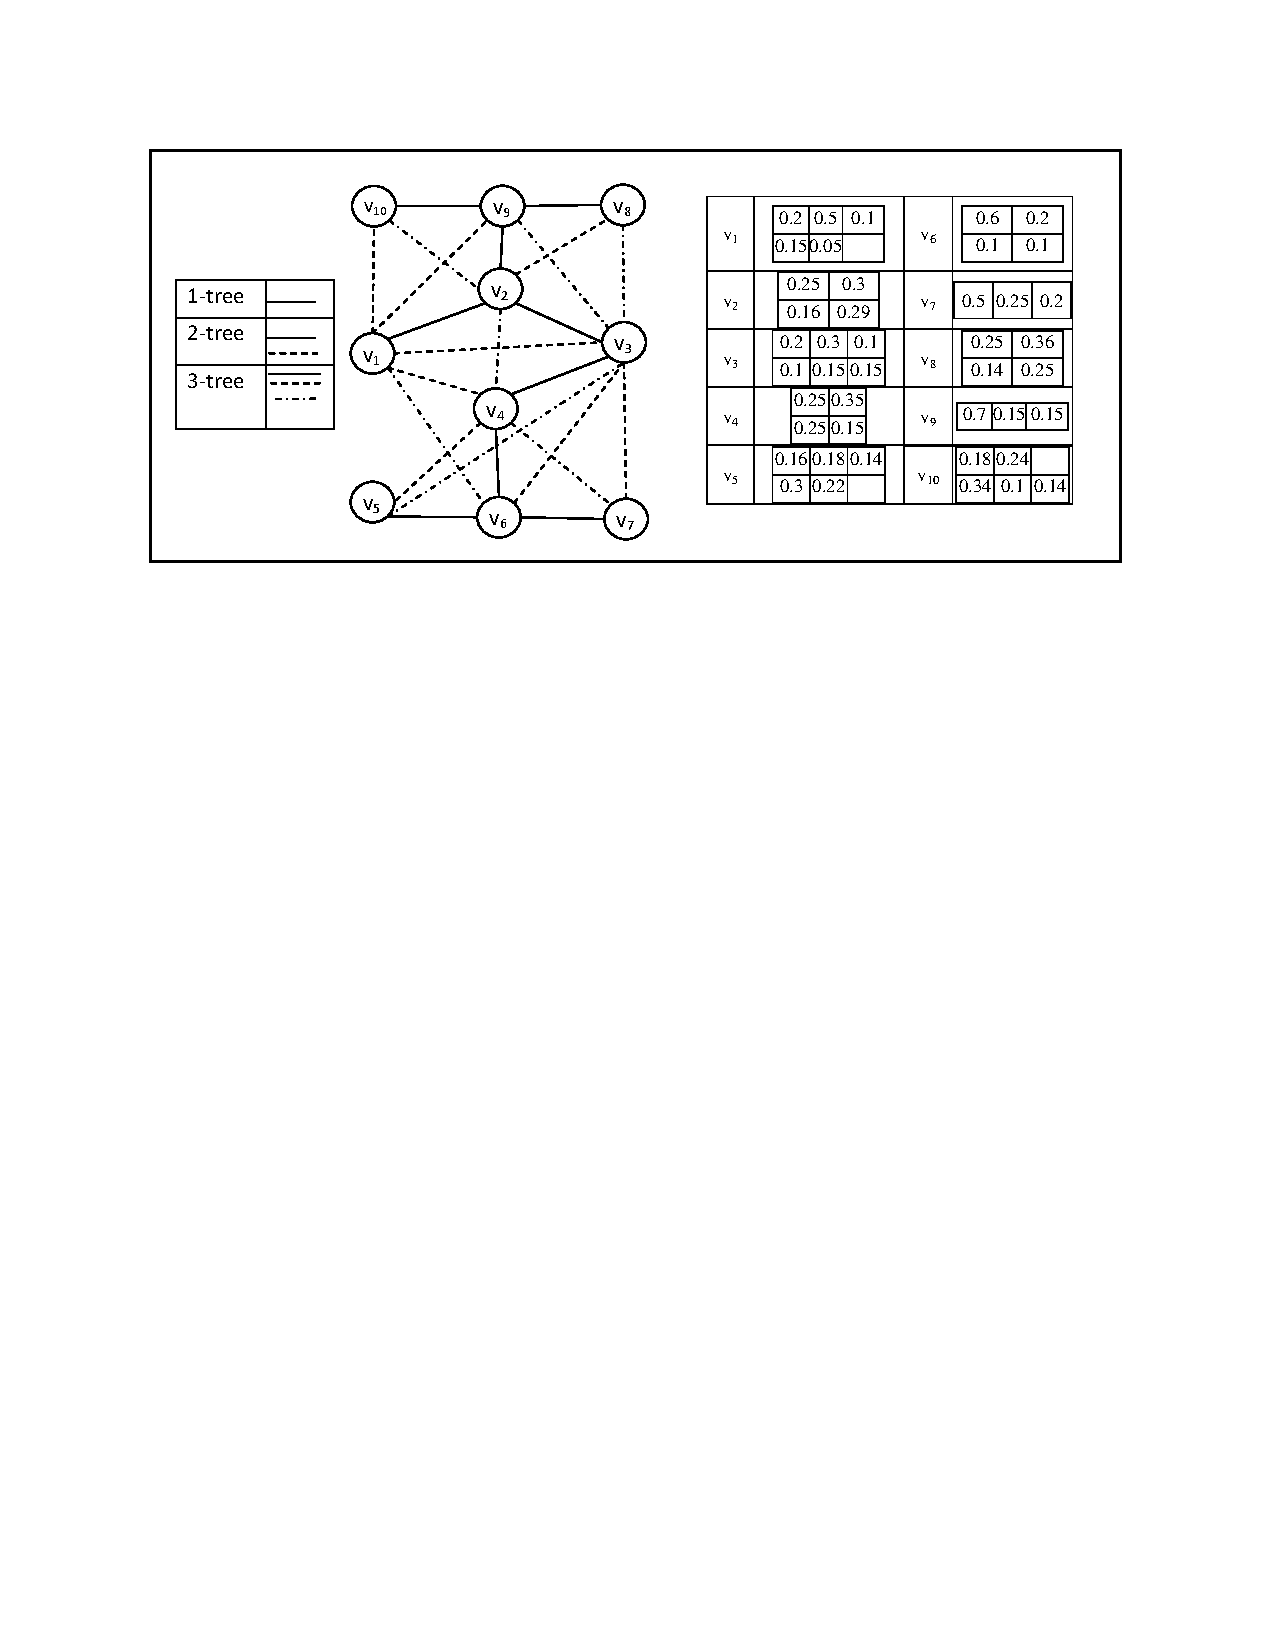
\includegraphics[width=6 in, height=2.8 in]{NetworkI_paper.pdf}
\caption{Network $G_{10}$}
\label{fig:netI}
\end{minipage}

\end{figure}
\begin{figure}[!htb]
\begin{minipage}{.9\linewidth}
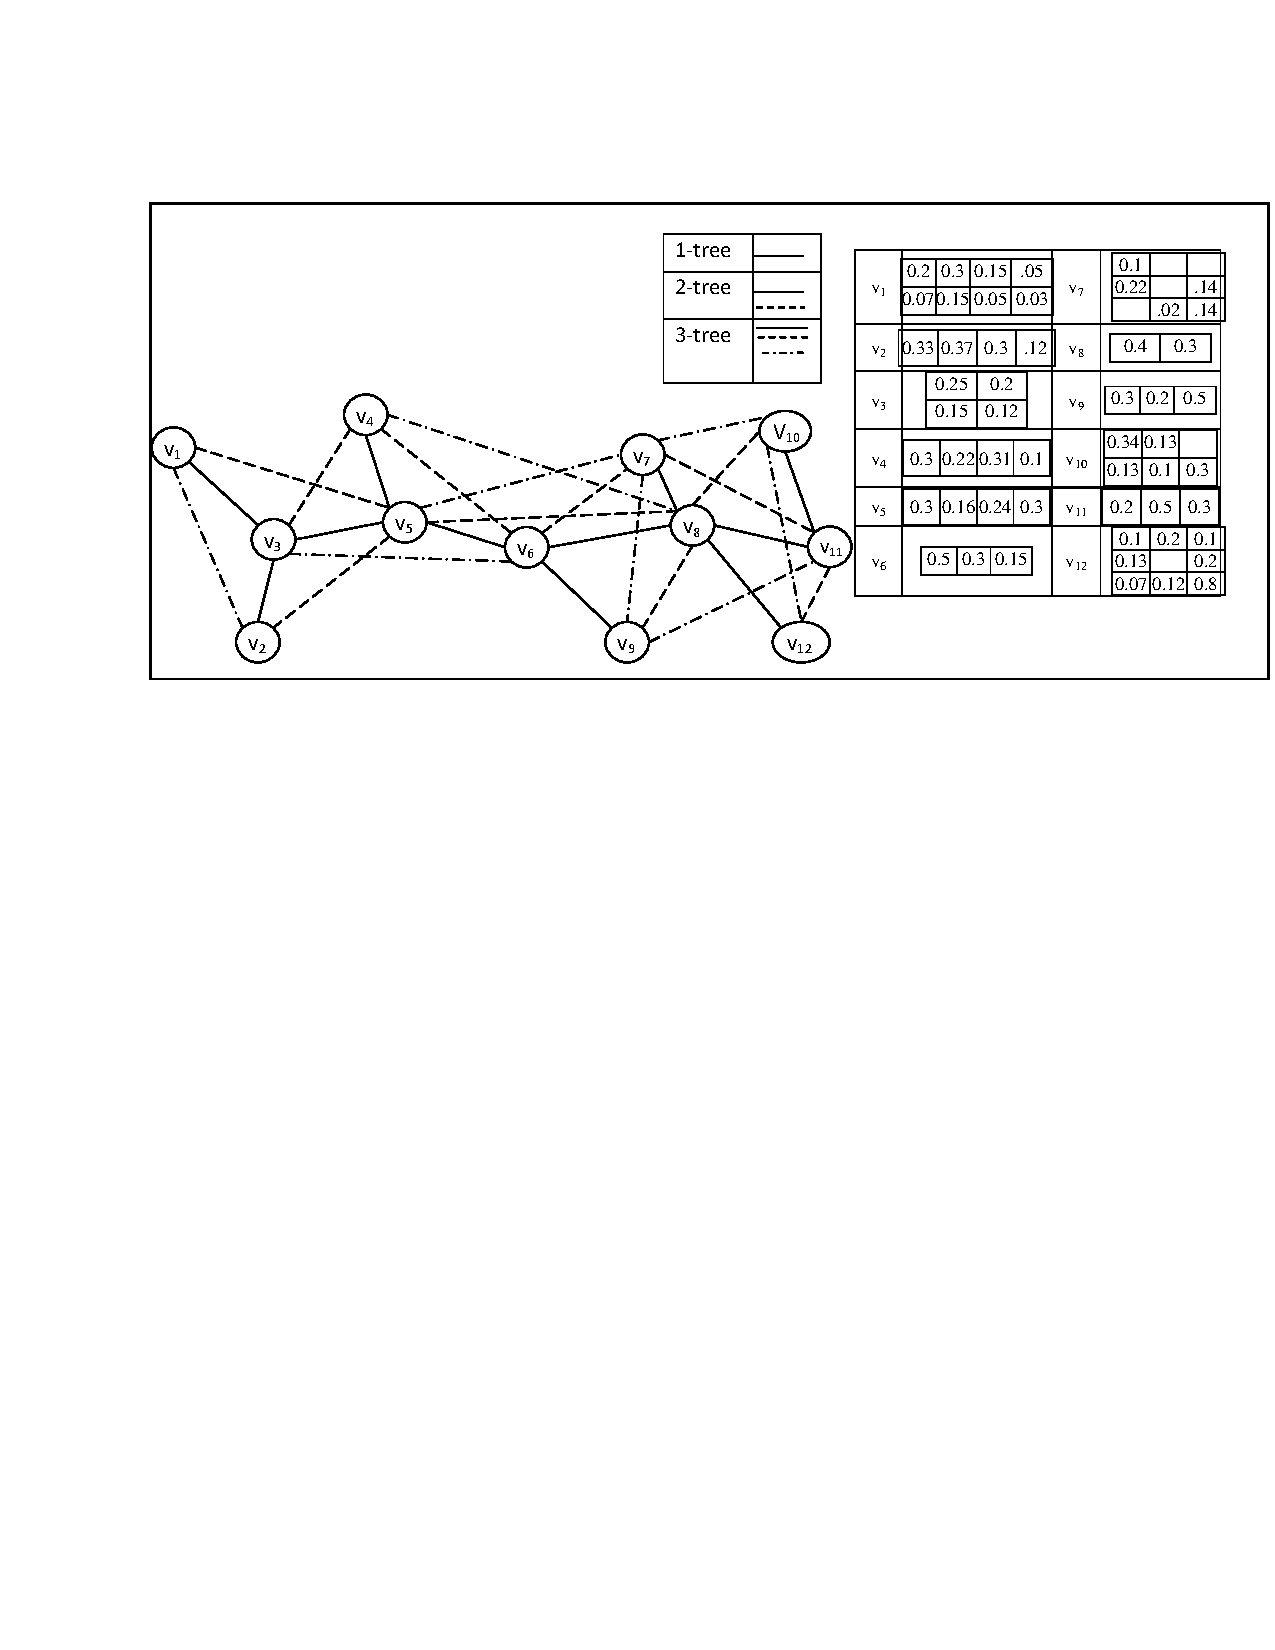
\includegraphics[width=6 in, height=2.7 in]{NetworkII.pdf}
\caption{Network $G_{12}$}
\label{fig:netII}
\end{minipage}
\end{figure}
\textbf{Test Networks:}
    For simplicity of constructing test networks and analyzing the obtained results, we assume that all nodes have the same transmission range $R_{tr}$, and we set the $E_G$ relation according to the Euclidean distance between the involved nodes.

We have experimented with networks of different sizes in the range $[7,18]$ nodes where each node has a locality set that varies in the range $[2,8]$ rectangles. Here, we  present results on three networks.
\begin{itemize}[noitemsep]
\item Network $G_{10}$ in figure \ref{fig:netI}, consists of $10$ nodes where the locality set of each node varies in the range $[4,6]$.
\item Network $G_{12}$ in figure \ref{fig:netII}, consists of $12$ nodes where the locality set of each node varies in the range $[3,8]$.
\item Network $G_{15}$ in figure \ref{fig:netIII}, consists of $15$ nodes where the locality set of each node varies in the range $[3,6]$.
\end{itemize}
The presented results highlight the most important findings. To avoid cluttering the network diagrams, we omit the $(x, y)$-coordinates of the locality sets. Solid lines in the figures indicate the links used in a spanning tree. Dashed links indicate links of  a 2-tree and dashed dotted links indicate links of a 3-tree.

\begin{figure}[!htb]
\begin{minipage}{.9\linewidth}
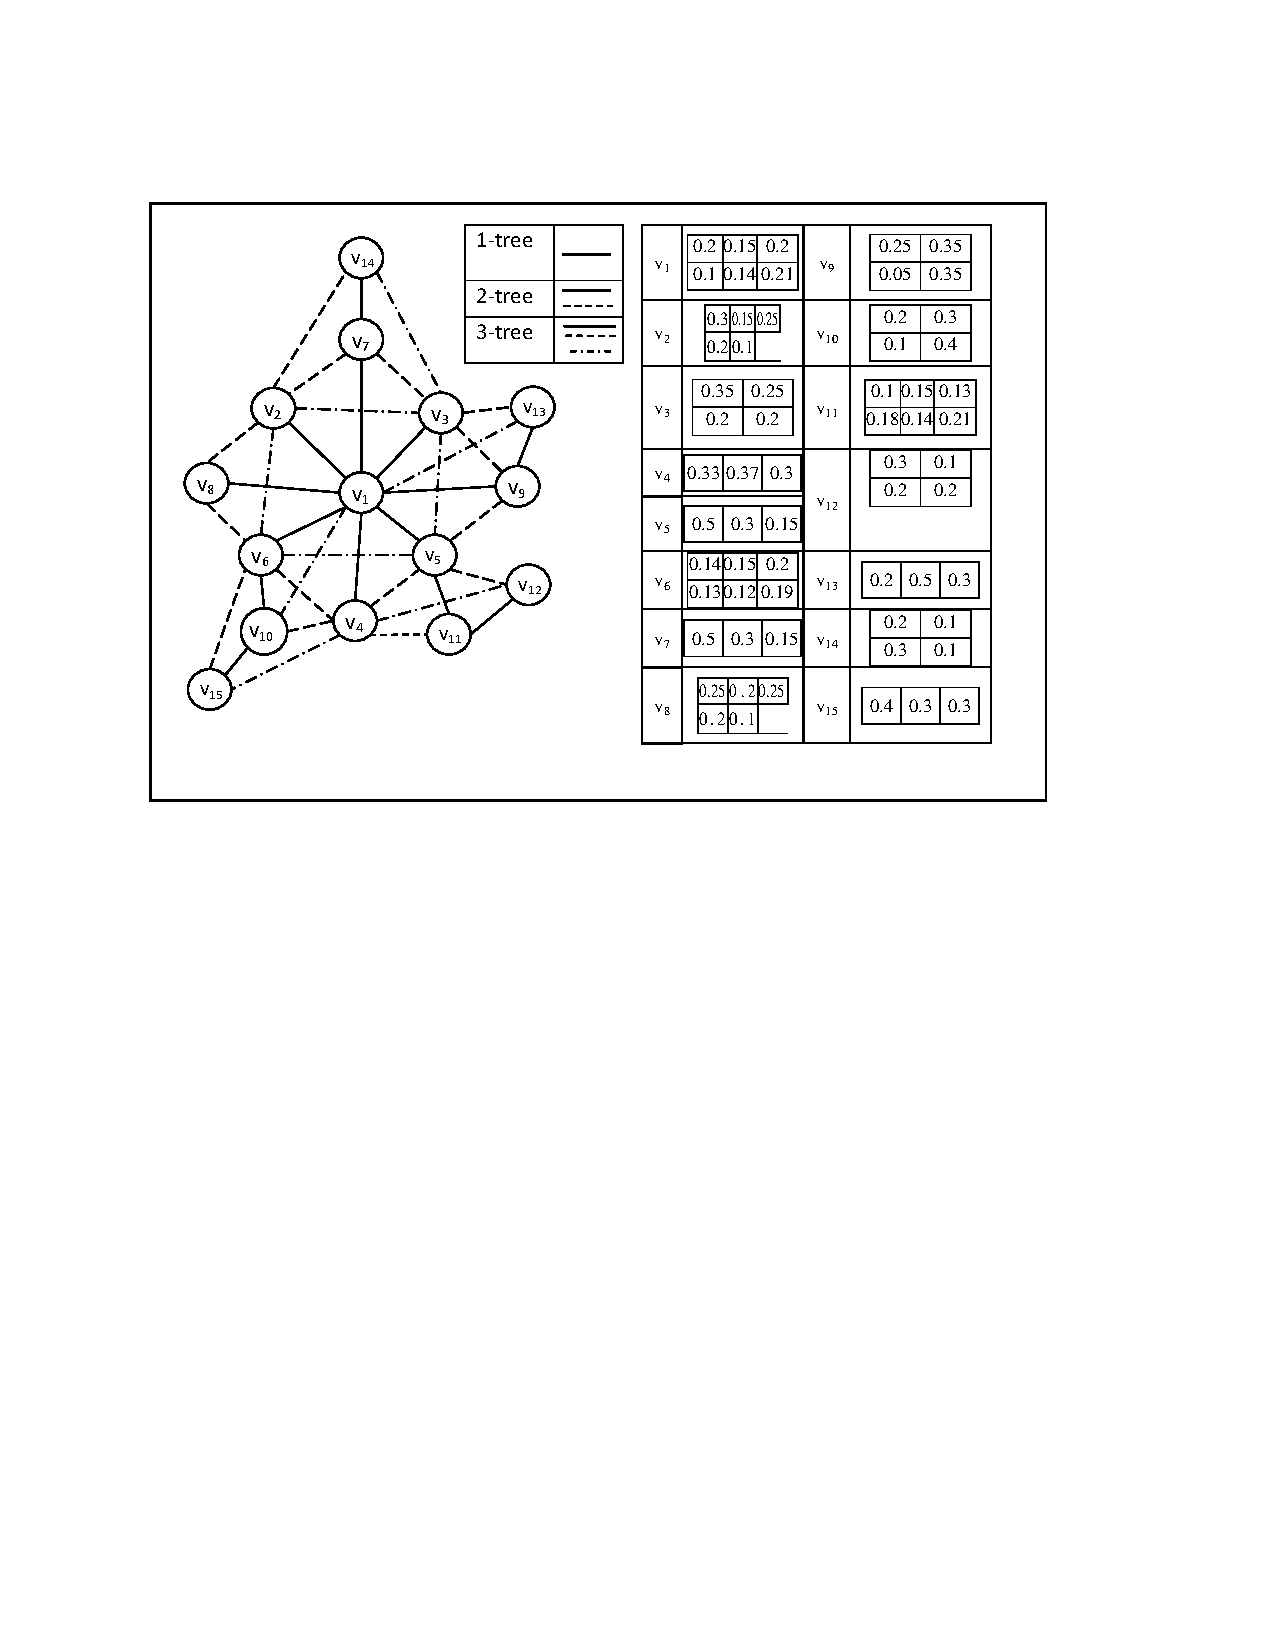
\includegraphics[width=6 in, height=2.6 in]{NetworkIII.pdf}
\caption{Network $G_{15}$}
\label{fig:netIII}
\end{minipage}
\end{figure}
   

\begin{enumerate}
\item \textbf{Running Time:} Table \ref{Tab:runtym} shows the obtained running time of the algorithm on each test network when the network is approximated by a tree (solid edges), 2-tree (solid and dashed edges), and 3-tree (all edges). As can be seen, processing 2-trees requires 10 to 15 times more time than processing trees. In addition, processing 3-trees may require 1000 times more time than processing 2-trees.

\begin{table}[!htb]

    %\caption{Global caption}
    %\begin{minipage}{.5\linewidth}
   
      \centering
     \begin{tabular}{|c|c|c|c|}
     \hline
         k& Network $G_{10}$ & Network $G_{12}$ & Network $G_{15}$ \\
     \hline
     1&90& 130& 200 \\\hline
     2&1000 &1380&1480	\\\hline
3 &60000&875000&940000	 \\\hline
\end{tabular}
 \caption{Running time in milliseconds}
\label{Tab:runtym}
\end{table}


\item \textbf{Effect of increasing the parameter $k$:}
Since the set of partial $k$-trees forms a proper subset of partial $k+1$-trees, one may expect that lower bounds obtained by using partial $k$-trees to be generally weaker than lower bounds obtained by using partial $k+1$-trees. This expectation is confirmed by the findings in table \ref{Tab:acc} constructed using networks $G_{10}, G_{12} \mbox{ and } G_{15}$. In the experiments, edges of the used tree, 2-tree, and 3-tree are computed using the greedy method. Table \ref{Tab:acc} indicates that for each of the 3 test networks, we have the following relation $\frac{Conn(\mbox{2-tree})}{Conn(\mbox{tree})}>\frac{Conn(\mbox{3-tree})}{Conn(\mbox{2-tree})}$.
 %\begin{minipage}{.5\linewidth}

   \begin{table}[!htb] 
      \centering
     \begin{tabular}{|c|c|c|c|}
     \hline
      k& Network $G_{10}$ & Network $G_{12}$ & Network $G_{15}$ \\
     \hline
      1 & 0.62&0.336& 0.82 \\\hline
2 &0.71 & 0.36& 0.99\\\hline
3 &0.75& 0.37& 1\\\hline
\end{tabular}
 \caption{Connectivity lower bounds using different partial $k$-trees}
 \label{Tab:acc}
\end{table}

\item \textbf{Effect of increasing node transmission range:} Intuitively, increasing node transmission range $R_{tr}$ of a given probabilistic network $G$ has two effects:
\begin{enumerate}
\item increasing the number of edges in the network and
\item increasing the probability that any given edge arises.
\end{enumerate}
 Consequently, denser partial $k$-tree subgraphs with better edge probabilities can be found. Thus, $Conn(G)$ is expected to increase. Figure \ref{fig:res} explores this aspect for network $G_{10}$ when $R_{tr}$ varies in the range $[5.5, 9.5]$ and a tree (partial 2-tree, or 3-tree) subgraph is selected randomly. As can be seen, bounds obtained by using a tree (2-tree, or a 3-tree) increases as $R_{tr}$ increases.

\begin{figure}[!htb]
\begin{minipage}[]{.5\linewidth}
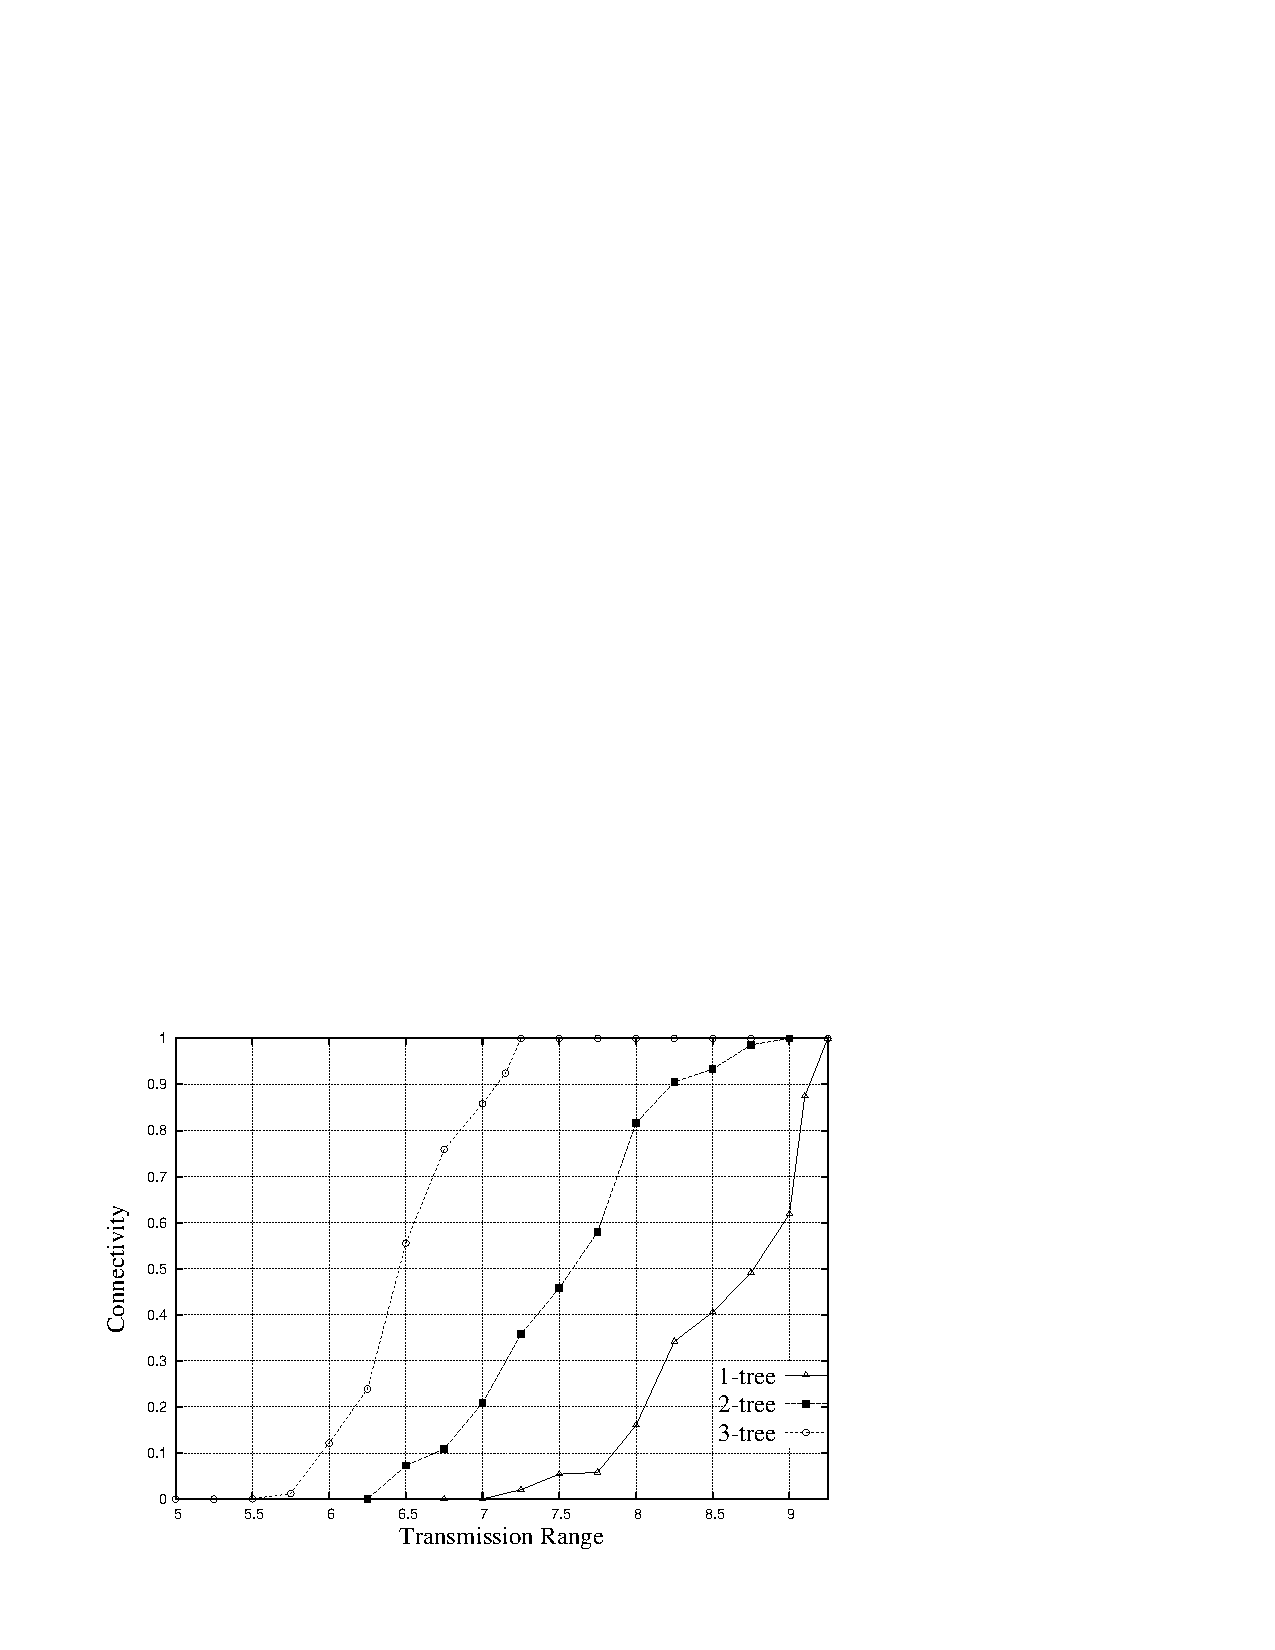
\includegraphics[width=3 in, height=2.5 in]{random1.pdf}
 \caption{ Connectivity versus transmission range with random subgraph selection}
\label{fig:res}
\end{minipage}
\begin{minipage}{.5\linewidth}
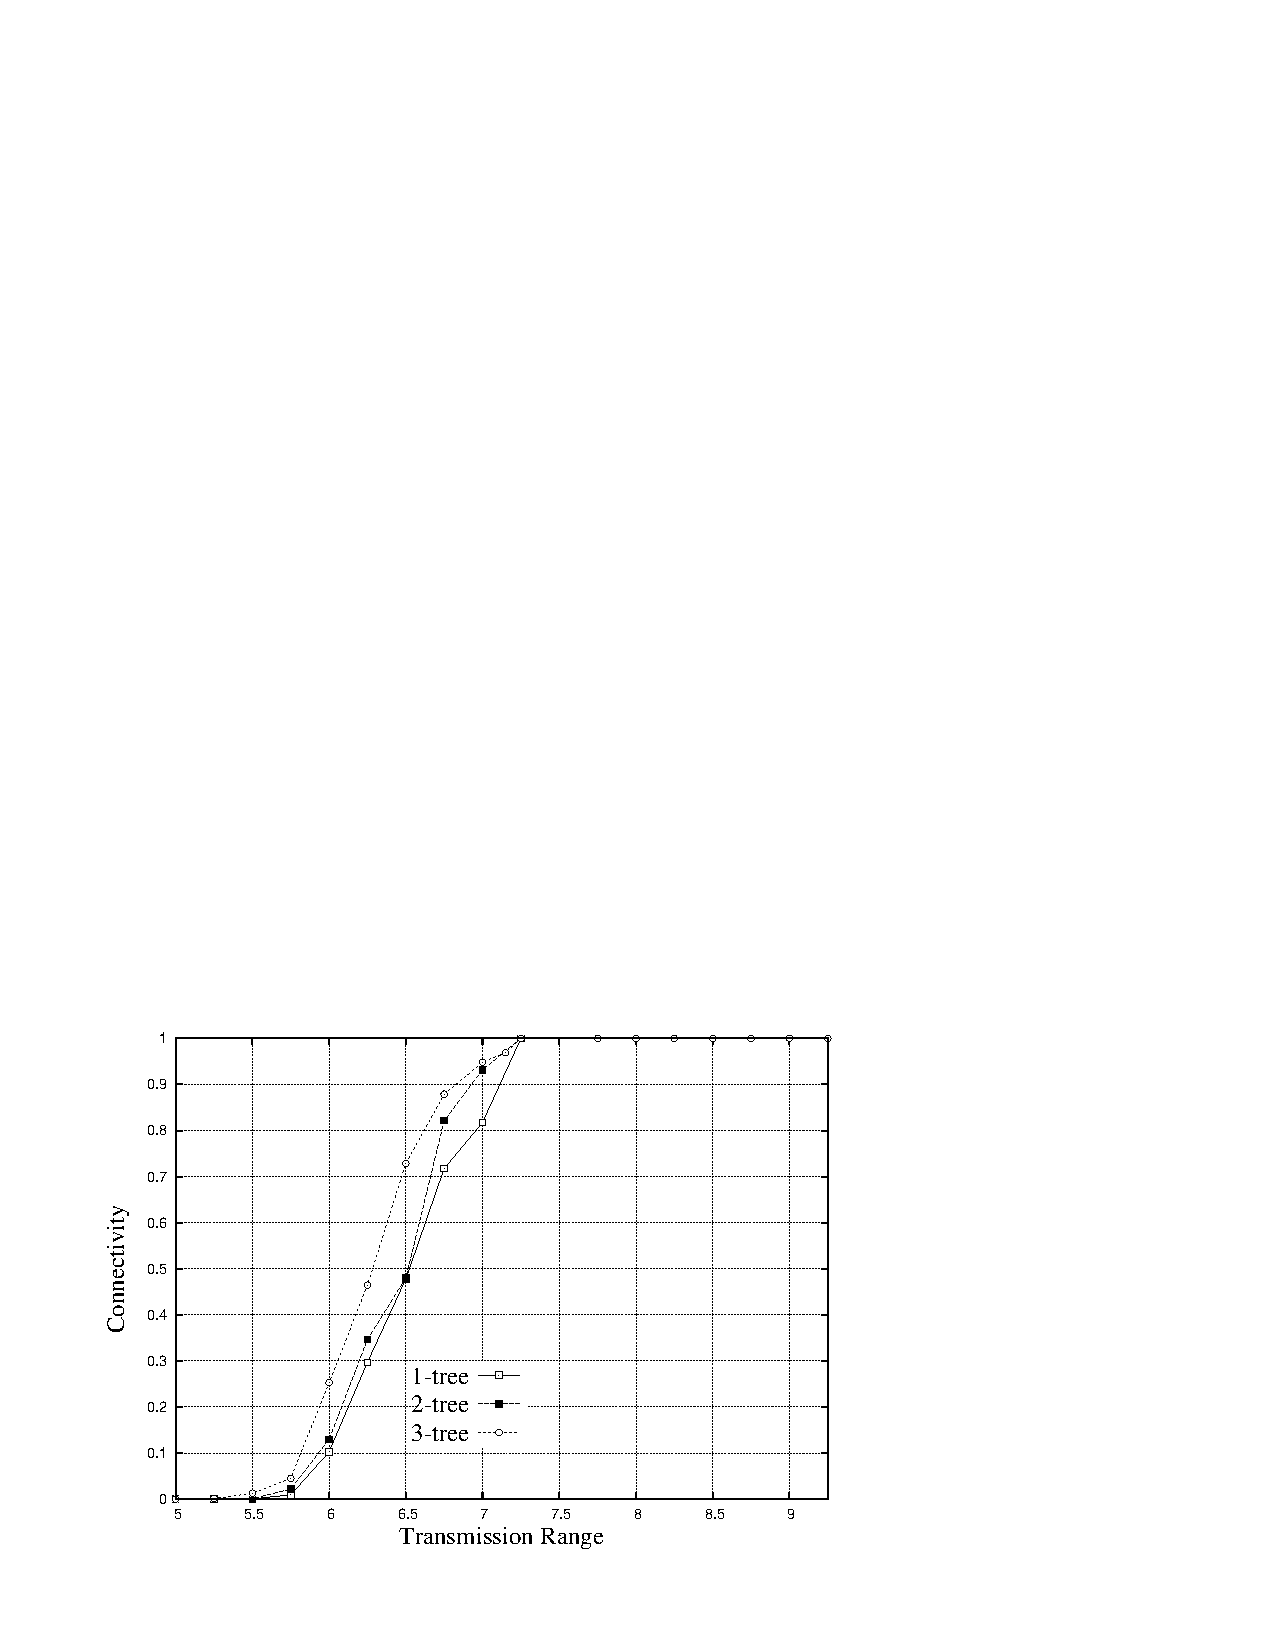
\includegraphics[width=3 in, height=2.5 in]{selective1.pdf}
 \caption{ Connectivity versus transmission range with greedy subgraph selection}
\label{fig:ges}
 \end{minipage}
\end{figure}

%\begin{figure}[!htb]
%\begin{minipage}[]{1\linewidth}
%\includegraphics[width=6 in, height=2.5 in]{output.pdf}
% \caption{ Connectivity versus transmission range with  random edge selection.
%}
%\label{fig:res}
%\end{minipage}
%\end{figure}
\item {\bf Effect of subgraph selection method:} Intuitively, for any given $k$, lower bounds obtained from partial $k$-tree subgraphs obtained using the greedy method (c.f. Chapter 2) are likely to be better than lower bounds obtained using the random method. To investigate this aspect, we compute lower bounds on network $G_{10}$ (used to generate figure \ref{fig:ges}) when we use partial $k$-tree subgraphs computed using the greedy method. The obtained results confirm the above intuition. For example, consider the bounds obtained by using tree subgraphs when $R_{tr}=6$. For this scenario, figure \ref{fig:res} gives  $Conn(G)\geq 0$ whereas figure \ref{fig:ges} gives $Conn(G)\geq 0.1$
\end{enumerate}



\section{Concluding Remarks}
In this chapter, we have extended the dynamic programming approach used in Chapter 3 to handle the $\ACONN$ problem on any probabilistic network whose underlying graph is a partial $k$-tree $G$, assuming that a $PES$ of $G$ is given. The algorithm runs in polynomial time for any fixed $k$. It provides a network design tool for analyzing probabilistic connectivity when any combination of the following parameters change: node locality sets, their probabilistic distribution, and node transmission range.    